%!TEX TS-program = xelatex
\documentclass[12pt]{./tex/thesis-umich}

\usepackage{acronym}
\usepackage{amsmath}
\usepackage{amssymb}
\usepackage{bm}
\usepackage{graphicx}
\usepackage{xcolor}
\usepackage{mathspec}
\usepackage{cite}
\usepackage{scalefnt}
\usepackage{booktabs}
%\usepackage{xfrac}
%\usepackage{listings}

\defaultfontfeatures{Mapping=tex-text, Ligatures={Common}}
\setmainfont{TeX Gyre Termes}
\setsansfont{TeX Gyre Heros}
\setmonofont{TeX Gyre Cursor}
\setmathfont(Digits,Latin,Greek){TeX Gyre Termes}

\title{Population Kinetics of a Repetitively-Pulsed Nanosecond Discharge}
\author{Benjamin T. Yee}
\department{Nuclear Engineering \& Radiological Sciences}
\year=2013

\frontpagestyle{1}

\dedication{ %
  I would like to dedicate this dissertation to someone else.
}

\acknowledgments[6]{ %
  Who is this?
}
\acknowledgmentswidth{0.8}

\preface[2]{ %
  This is a dissertation about something; I really hope it's good.
}

\committee{ %
  Associate Professor John E. Foster, Chair \\
  Doctor Edward V. Barnat, Sandia National Laboratories \\
  Doctor Isaiah M. Blankson, National Aeronautics and Space Administration \\
  Professor Augustus Evrard \\
  Professor Mark J. Kushner \\
}

\chair{John E. Foster}

\showlistofappendices

\abbreviations{ %
  \acro{rpnd}[RPND]{repetitively-pulsed nanosecond discharge}
\acro{dbd}[DBD]{dielectric-barrier discharge}
\acro{app}[APP]{atmospheric-pressure plasma}
\acro{lte}[LTE]{local thermodynamic equilibrium}
\acro{eedf}[EEDF]{electron energy distribution function}
\acro{fiw}[FIW]{fast ionization wave}
\acro{las}[LAS]{laser-absorption spectroscopy}
\acro{lif}[LIF]{laser-induced fluorescence}
\acro{lcif}[LCIF]{laser collision-induced fluorescence}
\acro{mhd}[MHD]{magnetohydrodynamic}
\acro{fwhm}[FWHM]{full-width half maximum}
\acro{fid}[FID]{fast ionization dynistor}
\acro{mipt}[MIPT]{Moscow Institute of Physics and Technology}
\acro{ccd}[CCD]{charge-coupled device}
\acro{ptfe}[PTFE]{polytetrafluoroethylene}
\acro{pic}[PIC]{particle-in-cell}
\acro{nasa}[NASA]{National Aeronautics and Space Administration}
\acro{grc}[GRC]{Glenn Research Center}
\acro{mmw}[mmW]{millimeter-wave}
\acro{emi}[EMI]{electromagnetic interference}
\acro{pmt}[PMT]{photomultiplier tube}
<<<<<<< HEAD
=======
<<<<<<< HEAD
\acro{gui}[GUI]{graphical user interface}
=======
>>>>>>> 156f02797d661c58657ab4a0a9c1df64db718d00
>>>>>>> bd734f46453e7c20bf9461d808ef12f216a035c0

}

\newcommand{\kB}{k_\mathrm{B}}
\newcommand{\dwa}{\Delta \omega_a}
\newcommand{\dwd}{\Delta \omega_d}
\newcommand{\nint}{\langle N \rangle}
\newcommand{\odd}{^\mathrm{o}}
\newcommand{\EE}{\times10^}


\begin{document}
  \chapter{Introduction}\label{chp:introduction}
    \section{Overview}

Historically, the study of atmospheric-pressure plasmas (\acs{app}'s) is
indistinguishable from the study of plasmas as a whole. However, the detail of
the measurements and calculations associated with \acs{app}'s has been limited
by their complexity. From a computational perspective, the high pressure and
number of potential reactions present a difficult challenge. Likewise, the high
pressure can significantly complicate the data analysis for a number of plasma
diagnostics. Aside from the high pressures, the large electric fields, short
time scales, and general randomness of \acs{app}'s make even the most basic
observations a feat.

In the last several decades, some of this has begun to change. High-powered
computing has allowed simulations with remarkable detail. Similarly, advances in
technology has enabled plasma diagnostics in regimes that were experimentally
inaccessible. As a result, the body of knowledge regarding \acs{app}'s has
greatly increased. Sometimes, the motivation for this work is scientific
curiosity. More often, the study of \acs{app}'s has been driven by a broad range
of applications.

Among the first plasma applications were provided by \acs{app}'s: ozone
generation and lighting. Aside from these items, plasma welding, polymer
treatment, combustion, and plasma televisions have become widely accepted.
Meanwhile, a large number of new applications may soon be added to this list,
including: treatment of tissue wounds, altering airflow over airfoils, and
destruction of industrial pollutants.

Unsurprisingly, each case demands a different kind of plasma. The original arc
discharges were created between two graphite rods connected to immense battery
banks. In contrast, a modern research reactor studying plasma-assisted
combustion might use a fast-switching semiconductor circuit. Over the years,
several types of \acs{app}s have been developed for a variety of situations:
dielectric-barrier, corona, thermal arc, RF, microwave, pulsed, and more.

Within this group\footnote{The interested reader is referred to Starikovskaia's
review \cite{Starikovskaia2006} which provides a general overview of \acs{app}'s
in the context of plasma-assisted combustion}, the repetitively-pulsed
nanosecond discharge (\acs{rpnd}) has created considerable interest. Generally
speaking, a \acs{rpnd} is a plasma generated by a repetitive electrical pulse
applied between two electrodes. The pulse voltage is often in excess of one
kilovolt, lasts anywhere from $<1-100$ ns, and is repeated over a thousand
times each second. The result is a wave of ionization (and light) which crosses
from the powered electrode to the grounded one.

A \acs{rpnd} can fill volumes of several liters with a relatively uniform
plasma. Though they can cause significant excitation of the background gas, they
generally produce very little heating (in some cases below a detection limit of
$\Delta \pm 15$ K). In addition, the excitation can be changed with adjustments
to the magnitude or duration of the electrical pulse. Each of these
characteristics are highly desirable in one or more of potential applications
for \acs{app}'s.

Given all of these promising properties, \acs{rpnd}'s have been the subject of
substantial study by several research groups. However, much of this work has
focused on the physics of \acs{rpnd}'s in air. Unfortunately, air's large number
of constituent elements can lead to notable complexity. In turn, this can
obscure some of the more fundamental questions relation to \acs{rpnd}'s: how do
they form, how is the energy distributed between excited particles, and what
kind of spatial variation can be expected?

This paper details a study of each of these questions in a helium \acs{rpnd}.
Specifically, the densities of one particular excited atom are measured for a
variety of pressures and locations. This is complemented by measurements of the
light emissions for the same set of parameters. A simple model of a \acs{rpnd}
is used to predict several characteristics of the plasma based on the excited
state densities: electron density, electric field, and light emission. The
measured light emissions are interpreted to show how the energy is distributed
in the gas, and how it changes over time. Finally, they are compared with the
estimated light emissions to check the validity of several common assumptions.

\section{Literature Review}

\acs{rpnd}'s are only a recent invention which resulted from advances in
fast-switching semiconductors. However, the physics of their formation is
related to a much larger category of plasmas which includes lightning, sparks,
and even some transient phenomena in DC glows. These plasmas are unique in that
their formation occurs on timescales much faster than the traditional Townsend
mechanism allows for. The means by which these plasmas form has acquired several
names in the literature; here we will adopt the term, fast ionization wave
(\acs{fiw}).\footnote{It should be noted that the phrase wave does not indicate
any kind of periodic motion or spatial arrangement. Simply put, it describes a
boundary which separates ionized and unionized gas which travels from one
electrode to another.}.

\subsection{Early History of Pulsed Discharges}

The first \acs{fiw} was likely generated by Wheatstone in 1835
\cite{Wheatstone1835}. As reported by Thomson \cite{Thomson1893}, Wheatstone
built a vacuum tube six feet in length, and applied a high voltage across the
gas. As a plasma formed in the tube, Wheatstone observed its formation with a
rotating mirror. The use of this apparatus allowed Wheatstone to place a lower
limit on the speed with which the plasma travelled from one electrode to the
other. Though the discharge crossed the tube with a speed of at least
$8\times10^7$ cm/s, spectral observations indicated that the particles emitting
the light were not travelling at that speed \cite{Zahn1879}.

Later, Thomson revisited this work with an improved apparatus
\cite{Thomson1893}. This included a tube that was now 15 m in length and five mm
in diameter, as seen in figure \ref{fig:thomson}.
\begin{figure}
  \centering
  \includegraphics[width=4in]{chapters/introduction/figures/thomson.png}
  \caption{A sketch of J.J. Thomson's early experiments on fast ionization
  waves in long vacuum tubes.}\label{fig:thomson}
\end{figure}
Also using the rotating mirror apparatus, Thomson was able to greatly improve on
the estimates of Wheatstone. He estimated that the so-called ``luminous front''
had a speed that was more than $1.5\times10^{10}$, or in excess of half of the
speed of light. Furthermore, Thomson determined that the front always appeared
to travel from the positively pulsed electrode (anode) to the ground electrode
(cathode).

The study of these luminous fronts was revisited by several researchers in the
wake of Thomson \cite{James1904, Whiddington1925, Beams1926} with varied
success. By his own admission, Beams's work in 1926 was done ``hurriedly,''
using a rudimentary Kerr cell. In 1930, Beams returned to the propagation of
light pulses in vacuum tubes with a rotating mirror apparatus \cite{Beams1930}.
In addition to confirming his previous measurements, and those of Thomson, Beams
discovered that the \acs{fiw} always traveled from the electrode with the
highest absolute potential, to the lowest one. In other words, the wave could be
anode or cathode directed, depending on the magnitude of their potentials
relative to ground. Benefiting from an improved understanding of electricity,
namely the existence of electrons and ions, Beams was able to provide the first
hypothesis on the nature of the \acs{fiw}:
\begin{quote}
  In the neighborhood of the electrode $\ldots{}$ the field is very high and
  intense ionization should take place. This ionization due to the large
  difference in mobilities of positive ions, negative ions and electrons
  respectively should result in the establishment of a space charge. This space
  charge, once formed near the high potential electrode $Q$ must move down the
  tube regardless of the polarity of the applied potential because of the
  changes it produces in the field near its edges.
\end{quote}

At about the same time, Schonland and Collens reported on their observations of
lightning \cite{Schonland1933}. Though the general structure and length scale of
lightning is substantially different from the luminous fronts observed by Beams
and Thomson, the two phenomena would later prove to be very similar. In their
work Schonland and Collens noted that lightning would usually occur in a
two-step process. Based on the images they obtained, they suggested that
the leader was generated by a relatively small ``dart'' with a mean vertical
velocity of $7.2\times10^8$ cm/s. The dart moved in a random manner, changing
directions at random intervals, but always moving downward.

The second step began when this dart reached the ground. Once there, a bright
return stroke would occur along the same path that the leader had traced out. In
contrast to the leader stroke, the return stroke had a velocity of $5\times10^9$
cm/s. Schonland and Collens hesitantly attributed the leader stroke to an
extended electron avalanche, and the return stroke to thermal ionization along
the conductive path generated by the dart. However, calculations by Cravath and
Loeb showed that the speeds of the proposed avalanche would have to be
inconsistent with the fields at the head of a lightning stroke
\cite{Cravath1935}. Instead, they suggested that the dart was actually a moving
region of space charge which locally accelerated electrons to ionizing energies.
This was fundamentally similar to the mechanism proposed by Beams in 1930.

\subsection{The Streamer Model}

It was long known that sparks in air were similar to lightning. Advances in
technology during the 1930's led to experiments which reinforced this
similarity. In response to the measurements of Schonland and Collens; Snoddy,
Beams, and Dietrich studied the breakdown of gas in a long tube with an
oscillograph \cite{Snoddy1936}. The results from the oscillograph showed a very
clear return wave for which they measured several parameters the characterized
as a function of pressure and applied potential. They observed that at low
voltages, the system behaved like a large resistor in series with a capacitor,
and below a critical voltage, no return stroke would form. Finally, in order to
explain the propagation of the \acs{fiw} generated by the positive pulse, they
suggested that photoionization was occurring in the space ahead of the wave.

Around the same time, Flegler and Raether had come to a similar conclusion,
leading to the first attempt at a theory describing streamers
\cite{Flegler1936}. This same theory was proposed independently by Loeb and Meek
in a series of papers \cite{Loeb1940, Loeb1940a, Meek1940}. The streamer theory
divided the initial breakdown of a spark into two steps. In the first step, an
electron avalanche is initiated between two electrodes. The avalanche travels
toward the anode and leaves behind a region of high positive space charge. In
the second step, the return stroke begins at the cathode and travels toward the
cathode. It was suggested that the head of the return stroke ionizes the gas
ahead of it by pulling in background electrons or via photoionization.
\footnote{These early works emphasized the importance of photoionization. It is
now know that it is only required for cathode-directed streamers in systems with
no background ionization. In addition, Mesyats later showed that the lifetime of
the excited states responsible for photoionization were often longer than the
lifetime of the streamers \cite{Mesyats1972}}.

The streamer model proved relatively successful in describing the development of
sparks and lightning. Theoretical estimates of the speed matched the velocity
measurements that were acquired through photographs and oscillographs.
Additionally, the theory is able to account for the halting manner in which
lightning is formed, though it is only tentatively able to describe the
branching and stepped appearance. Finally, the streamer mechanism provides an
adequate explanation of why streamer discharges are not affected by the shape or
material of the cathode, namely, they do not depend on secondary electron
emission.

The study of the formation of streamers and lightning continues to be active to
this day. Following the initial work of Flegler, Raether, Loeb, and Meek, a
number of researchers began to explore the boundary between the Townsend
mechanism and the streamer mechanism. Most notable was Fisher and Bederson's
work in 1951 \cite{Fisher1951}, which was later extended to nitrogen
\cite{Kachickas1952} and argon \cite{Kachickas1953}. However, there were still a
number of phenomena that were poorly explained by the streamer model. In
particular, Kunhardt provided a useful overview of the problems in 1980
\cite{Kunhardt1980}. However, even before that, it was apparent that the
transients of sparks and lightning was more complicated than thought.

\subsection{Ionizing Waves of Potential Gradient}

Per Chalmers \cite{Chalmers1971}, Rogowski and Buss \cite{Rogowski1927,
Buss1932} observed a fast, diffuse, glow discharge immediately prior to the
filaments which often accompany a streamer discharge. Allibone and Meek, noted
similar diffuse discharges in air based on oscillographs and photographs
\cite{Allibone1938, Allibone1938b, Allibone1938c}. However, the Boys apparatus
which was employed in these studies (an ancestor to the modern streak camera)
was unable to capture the evolution of the diffuse glow, given its large spatial
extent.

This was first noted by Allibone who attempted to use Lichtenberg
figures\footnote{Such figures directly exposed photographic emulsions to the
electrical discharge. The developed image was a time-integrated representation
of the discharge.} to definitively capture this diffuse glow
\cite{Allibone1948}. Later, Saxe and Meek used the recently invented
photomultiplier tube to record the evolution of the light emissions in the
brief, diffuse glow \cite{Saxe1948} as a function of space. Both studies
agreed in the existence of the diffuse glow, despite some disagreement on the
nature of its geometry and propagation.

The similarity of fast transient ionization waves in certain glow discharges
\cite{Westberg1959} to those observed in lightning and streamers led Loeb to to
the conclusion that they were all the same phenomena \cite{Loeb1965}. He
referred to them as ``ionizing waves of potential gradient,'' as the proposed
mechanism for the waves was the generation of a steep potential gradient in a
sufficient short period of time. 

As reported by Babich, Loika, and Tarasova \cite{Babich1977}, the detection of
x-ray emissions from pulsed, high-pressure, helium discharges created a new
avenue of interest for these transient plasmas \cite{Stankevich1967,
Noggle1968}. Unlike the streamers, which were often filamentary, these new
discharges exhibited surprising uniformity. The primary difference being the
duration of the pulse (on the order of nanoseconds) and the applied potentials
(in excess of 200 kV).

The x-rays suggested that electrons in these discharges were accelerated to
unusually high energies (on the order of 10 keV) despite the high
collisionality. It was then that Babich and Stankevich suggested that the x-rays
resulted from continually accelerated electrons impinging on the metal
electrodes \cite{Babich1973}. Briefly, the electric fields in the fronts of the
ionizing waves were so large that they managed to accelerate electrons past the
peak in their collisional cross sections.

Mesyats, Bychov, and Kremnev attempted to provide a more rigorous explanation
for the uniform nature of these new discharges \cite{Mesyats1972}. After
conducting several experiments, they came to the conclusion that these transient
plasmas were the result of many overlapping avalanches, unlike the streamer
which only involves a single avalanche. Kunhardt and Byszewski later
expanded on this work by developing a kinetic model to explain the behavior of
all pulsed discharges above the Townsend threshold \cite{Kunhardt1980}.

It was based on the studies of the fast electrons in these discharges that
Mesyats, Bychov, and Kremnev proposed the use of a fast electron beam for
pumping high-pressure gas lasers. Similar work was conducted simultaneously by
Fenstermacher et al.~\cite{Fenstermacher1972}. Palmer \cite{Palmer1974}, and
Levatter and Lin \cite{Levatter1980} determined that there was a threshold
amount of preionization required to ensure homogeneity of the discharge. Hunter
\cite{Hunter1976}, and Koval'chuk and Mesyats \cite{Koval'chuk1976} later
proposed that such discharges be used for fast-closing switches. Gas lasers and
fast switches would drive much of the later research on fast, pulsed discharges.

Eventually these discharges came to be referred to as fast ionization waves
(\acs{fiw}s). A large body of Russian literature developed around their study,
though much of it has remained untranslated. In 1994, Vasilyak produced an
extensive review of these studies \cite{Vasilyak1994}. The data include wave
velocities for a variety of gases and pressures. Other parameters such as
attenuation coefficients for the waves, high energy electron currents, electric
field measurements, and a circuit model of the \acs{fiw} are also included.

\subsection{\textsc{rpnd}s}

Beginning in 1998, the Moscow Institute of Physics and Technology (\acs{mipt})
produced a flurry of studies on the \acs{fiw} \cite{Anikin1998, Pancheshnyi1998,
Starikovskaia1998}. They employed several different diagnostic techniques
(photomultiplier tubes and capacitive probes) in an exceptionally detailed study
in both air and nitrogen, using a shock tube and a bell jar. A summary of these
investigations can be found in \cite{Starikovskaia2001}. The work showed
exceptionally reproducibility of the discharge parameters at relatively low
repetition rates, on the order of tens of Hz, and evidence of runaway electrons.
This work also included some of the first approximations of the electron energy
distribution function (\acs{eedf}).

Interestingly, later analysis of a anode-directed \acs{fiw} in nitrogen by the
group at \acs{mipt} \cite{Pancheshnyi1999} concluded that the, the vast majority
of the electrons were generated \emph{after} the wave. This suggests that the
ionization in an \acs{fiw} does not strictly track the luminous front of the
wave. Additionally, measurements of the conductivity suggested that the local
approximation becomes invalid in the wave front and the electron energy
distribution function resembles a beam.

In 1997 the invention of the fast ionization dynistor (\acs{fid}) was revealed
\cite{Efanov1997}. These new devices enabled sub-nanosecond switching of 10's of
kilovolts, with repetition rates approaching 100 kilohertz. This was a leap
forward over previous technologies which generally used thyristors or spark gaps
for switching. Particularly appealing was the high repetition rate of the
\acs{fid}.

Recall that the volume-filling \acs{fiw} required a significant
amount of preionization. This was often accomplished an ionization source in
addition to the high voltage pulse (in the form of UV radiation, or electron
beams). However, the repetition rates of \acs{fid}s were high enough such that a
substantial number of electrons would carry over between pulses. These seed
electrons obviated the need for a preionization. In addition, the time-averaged
densities of excited states could maintained at much higher values. This had
particular promise for processing applications.

In the eventual commercialization of the \acs{fid} made economically feasible to
create fast, repeatable fast ionization waves. It is this class of discharges
which are now referred to as repetitively-pulsed nanosecond discharges, or
\acs{rpnd}s. Their uniformity, low gas heating, high-pressure operation, and
efficient ionization made them attractive or a number of applications:
\begin{itemize}
  \item plasma-assisted combustion \cite{Starikovskaia2006},
  \item magneto-hydrodynamic energy bypass \cite{Macheret2002},
  \item plasma actuators \cite{Adamovich2009},
  \item and high-pressure xenon lamps \cite{Nikandrov2008, Tsendin2009}.
\end{itemize}

As with the \acs{fiw}s, the primary diagnostics were current and voltage
characteristics, electric field measurements with capacitive probes, and
emission measurements with photomultiplier tubes. Later, intensified \acs{ccd}s
were used to record the emissions of specific transitions as well as broadband
light. This approach has been used to more clearly illustrate the uniformity and
reproducibility of the discharge \cite{Adamovich2009}. Other researchers have
turned to laser-based diagnostics, such as coherent anti-Stokes Raman
scattering, to measure gas heating \cite{Zuzeek2010} and the electric field in
molecular systems \cite{Ito2010, Ito2010a}. Likewise, laser collision-induced
fluorescence (\acs{lcif}) has been used to obtain axial profiles of excited
state and electron densities in helium \acs{rpnd}s \cite{Weatherford2012}.

Concurrent with these improvements in experimental techniques has been similar
progress in the simulation of \textsc{rpnd}s. The one-dimensional models 


  
  \chapter{Theory}\label{chp:theory}
    \section{Ionized Gas}
A plasma is considered to be a form or subset of ionized gas. That is, a
volume of neutral atoms or molecules, of which some fraction has been
separated into electrons and ions. For a sufficiently large number of
particles, the behavior of each species in the ionized gas can be
described by a continuous distribution function which specifies the
number of particles with a specific range of velocities, in a specific
volume, at a specific time. This function is denoted
$f_\alpha(\vec{r_\alpha}, \vec{v_\alpha}, t)$, where the subscript
$\alpha$ denotes the species, $f$ is the probability distribution,
$\vec{r}$ is the position, $\vec{v}$ is the velocity, and $t$ is the
time.

The behavior of $f_\alpha$ can be shown to be governed by the
Vlasov-Fokker-Planck (\acs{vfp}) equation,
\begin{equation}\label{eq:vfp}
  \frac{\partial f_\alpha}{\partial t} + \vec{v_\alpha}\cdot\nabla f_\alpha +
  q_\alpha \left(\vec{E} + \vec{v_\alpha}\times\vec{B}\right)
  \cdot \nabla_\mathrm{v} f_\alpha = \left( \frac{\partial f_\alpha}
  {\partial t}\right)_\mathrm{coll}.
\end{equation}
Here, $q$ is the charge of the species, $\vec{E}$ is the electric field,
$\vec{B}$ is the magnetic field, and $\partial f_\alpha/(\partial
t)_\mathrm{coll}$ is a term which represents changes to the distribution
function as a result of collisions. The \acs{vfp} is a rigorous kinetic
description of an ionized gas. Coupled with Maxwell's equations, it is
can provide a complete and self-consistent description of the particle
densities in an ionized gas as well as the electric and magnetic fields.

For a species in equilibrium in the absence of external forces
(($\partial f_\alpha/\partial t)_\mathrm{coll} = 0$) it can be shown
that
\begin{equation}\label{eq:mb}
  f_\alpha(v_\alpha) =
    n_\alpha\left( \frac{m_\alpha}{2\pi \kB T_\alpha}\right)^{3/2}
   \exp\left(-\frac{m_\alpha v_\alpha^2}{2\kB T_\alpha}\right),
\end{equation}
where $n$ is the total density of the species, $m$ is the particle mass,
$\kB$ is Boltzmann's constant, and $T_\mathrm{alpha}$ is the temperature
of the species. It must be emphasized that this solution only applies to
situations where the species can be considered to be in equilibrium.
Strong gradients and large electromagnetic fields can both drive a
distribution far from its equilibrium condition. This is particularly
important when plasmas are discussed in the context of temperature.

Solutions of the \acs{vfp} in anything but this simple case can be very
challenging. It most situations, it is reduced to more tenable equations
by integrating over the velocity-space (leaving $f$ as only a function of
space and time). The first so-called moment is often called the conservation
equation or continuity equation,
\begin{equation}\label{eq:cont}
  \frac{\partial n_\alpha}{\partial t} + \nabla \cdot (n_\alpha \vec{u_\alpha})
  = G_\alpha - L_\alpha.
\end{equation}
In this case, $\vec{v}$ has been replaced by a mean velocity $\vec{u}$.
We have also introduced terms losses ($L$) and gains ($G$) in the
species density.

The definition of the mean velocity can be obtained by multiplying the
\acs{vfp} equation by $v$ and integrating over velocity-space. This is
referred to as the second moment. The result is an equation expressing
the conservation of momentum for the species. The actual equation will
not be reproduced here, but it forms the basis for the two-fluid
approximation of a plasma. In the course of developing the second
moment an additional term, the pressure tensor, is introduced which can
only be defined by the third moment of the \acs{vfp} equation. In fact,
each additional moment introduces a new term, \emph{ad infinitum}. For
most cases, the first two or three moments suffice, after the sequence
is terminated by the use of an additional assumption.

For our purposes, one more moment will suffice. Multiplying by $mv^2/2$,
integrating over velocity-space, and assuming that the pressure is
isotropic, produces the energy conservation equation,
\begin{equation}
  \frac{\partial}{\partial t}\left(\frac{3}{2}p_\alpha\right) 
  + \nabla\cdot\frac{3}{2} (p_\alpha\vec{u}_\alpha)
  + p_\alpha\nabla\cdot\vec{u}_\alpha
  + \nabla\cdot\vec{q}_\alpha
  = \frac{\partial}{\partial
  t}\left(\frac{3}{2}p_\alpha\right)\bigg|_\mathrm{coll}.
\end{equation}
In this case, $p$ represents the plasma pressure, and $\vec{q}$ is the
heat flow. The first term on the \textsc{lhs} represents the total
energy contained by the species, the second term is the energy flux in
and out of the volume, and the third term accounts for changes due to
compression or expansion. The \textsc{rhs} is the collision operator
which describes energy added or removed from the system as a result of
collisions.

\section{Plasma Criteria}
Previously, it was stated that plasmas were a form of ionized gas. 

To a large extent, a plasma can be categorized based on its electron
temperature and density. Figure~\ref{fig:regimes}
\begin{figure}
  \centering
  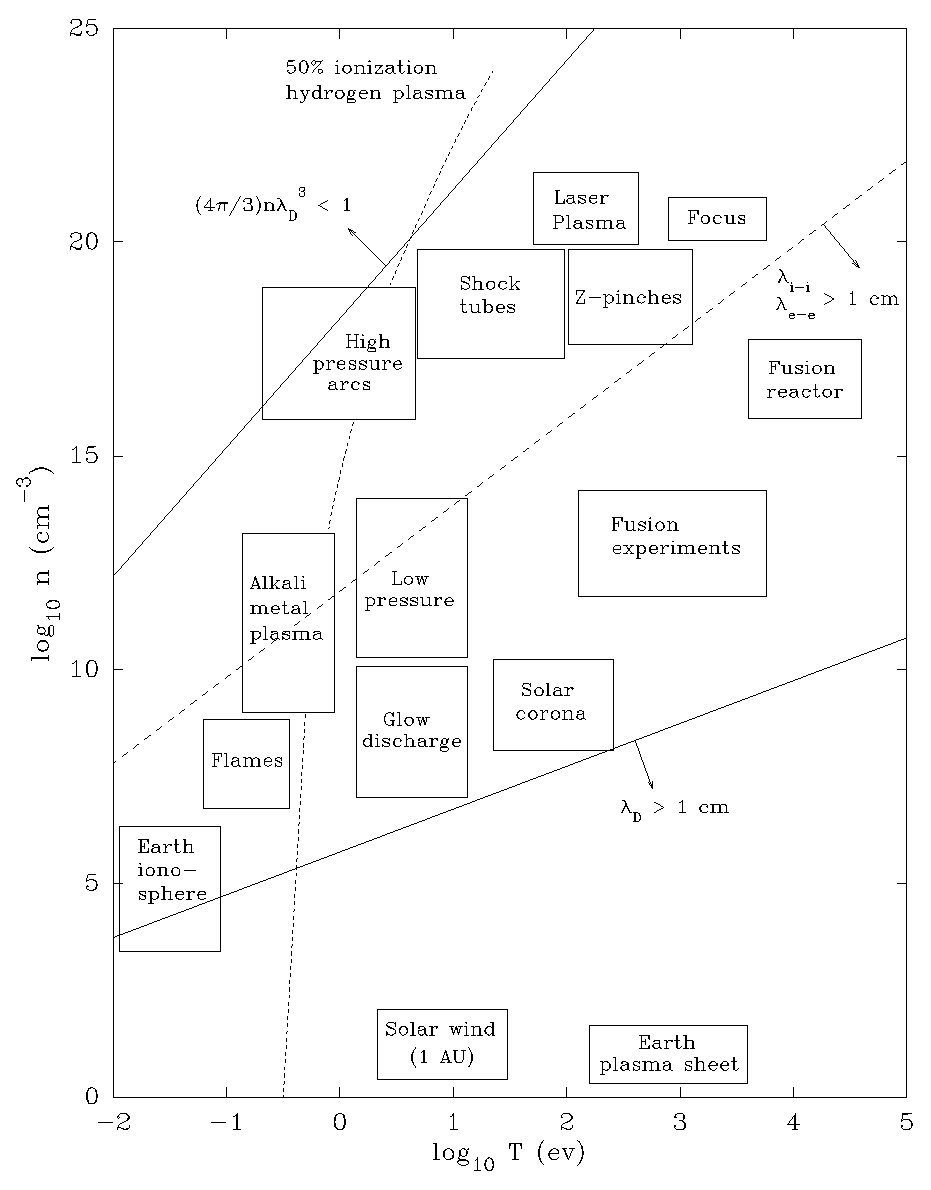
\includegraphics{./chapters/theory/figures/regimes.eps}
  \caption{Illustration of the various regimes of plasma in terms of
electron temperature and density \cite{Huba2011}.}
  \label{fig:regimes}
\end{figure}
shows where a number of different types of plasmas fall based on this
classification. As can be seen, the electron temperature of a plasma can
cross seven orders of magnitude, and the density can extend over 20.
While a plasma is often described as an ionized gas, the two are not
interchangeable; ionization of a gas is a necessary, but not sufficient
condition for a plasma. There are three additional criteria which are
used to identify a plasma.

\subsection{$\lambda_\mathrm{D} < L$}
An ionized gas is composed of both positive and negative charges,
usually ions and electrons, respectively. When an electrical
perturbation is introduced, the electrons and ions will arrange
themselves so as to screen or shield the perturbation. This causes the
electric field of the perturbation to fall off more rapidly than the
typical $r^{-2}$. The length scale of this shielding effect is referred
to as the Debye length, denoted $\lambda_\mathrm{D}$. The Debye length
can be shown to be equal to $\sqrt{\epsilon_0T_\mathrm{e}/(en_0)}$,
where $\epsilon_0$ is the vacuum permittivity, $T_\mathrm{e}$ is the
electron temperature, and $n_\mathrm{e}$ is the electron density.

\subsection{$n(4/3\pi r^3) >> 1$}
\subsection{$\omega_p > \nu$}

\section{Atomic Spectroscopy}

Spectroscopy spans a large body of theory which cannot be adequately
covered here. Given that the measurements are all for helium, we will
limit ourselves to a simple description of atomic spectroscopy. An atom
is made of positively charged nucleus and a number of negatively charged
electrons which orbit this nucleus. In the unperturbed, or ground state,
the electrons occupy orbitals determined by a full solution of the
Schrodinger equation.

However, interactions with other particles or photons can excite one or
more of the electrons into orbitals with higher potential energy. In
most cases relevant to low temperature plasmas, only a single electron
will be excited at any given time. Depending on which orbital the
electron is excited to, it can transition to orbitals with lower
potential energy by emitting a photon. These are typically called
allowed transitions.

Each orbital in an atom can be described by four quantum numbers.
\begin{itemize}
  \item $n$ - The principal quantum number.
  \item $l$ - Orbital angular momentum number.
  \item $j$ - Total angular momentum.
  \item $m_j$ - Total angular magnetic moment.
\end{itemize}
The Pauli exclusion principle restricts more than a single electron from
occupying any given state defined by this series of numbers.
Additionally, each set of numbers determines the potential energy
possessed by an electron in that particular level. 

Allowed transitions are determined by a series of selection rules. These
selection rules can be summed up as the following:
\begin{itemize}
    \item $\Delta S = 0$
    \item $\Delta L = \pm1$
\end{itemize}
Though other transitions are possible (spin and dipole forbidden respectively),
they tend to require an external perturbation in order to induce transition.

Figure shows the what is commonly called a Grotrian diagram for helium.
In this diagram, the vertical axis represents the energy above the
ground state, and the levels are arranged horizontally based on
increasing $L$. Levels which are radiatively linked are connected by
solid lines. As can be seen in this figure, only the levels having $S=1$
are radiatively connected to the ground state. As a result, any helium
atoms that are excited into the triplet manifold tend to stay there,
accumulating in the metastable state, $2^3S$.

Approaching 24 eV, the excited electron enters what is known as the continuum.
The energy separation between states goes as $n^{-2}$, thus at large $n$ the
spacing becomes quite close and the states are almost indistinguishable. The
levels are often referred to as Ryberg states. Above 24.69 eV, the electron
becomes totally detached from the helium nucleus, and all that remains is
a singly ionized helium atom.

Though the emissions of ions can be quite useful in some plasmas, we do not
concern ourselves with them in either the measurements or models. 24.69 eV is
the largest known ionization potential, and as a result, the number of ions and
the emissions associated with them remain relatively small.

\subsection{Spectral Lineshapes}
It is tempting to think that the energy spacing can be calculated exactly,
however there is always some variance about a central energy. This is called the
spectral lineshape, and it effects both the energy of the emitted photon in
radiative transitions, and the photons that an atom can absorb. Though these
variations can be attributed to quantum mechanical effects, the actual result
can derived from the so-called dipole approximation.

In this case, we envision a single electron oscillating about a large, heavy,
positive charge. The full details of this derivation are covered in Siegman
\cite{Siegman1986}, however we'll address some of the most pertinent portions
here. The response of a collection of atoms to an applied electric field can be
expressed as a quantity known as the susceptibility. This is generally defined
as
\begin{equation}
    \tilde{\chi}(\omega) \equiv
    \frac{\tilde{P}(\omega)}{\epsilon_0\tilde{E}(\omega)}
\end{equation}
where $\tilde{\chi}$ is the electric susceptibility, $\tilde{P}$ is the
macroscopic polarization, $\tilde{E}$ is the applied electric field, and
$\omega$ is the frequency of the applied field.

\paragraph{Natural Linewidth}
The electric susceptibility often possesses both a real and imaginary component.
Physically, these respectively represent the reactive and absorptive component
of the medium. Accounting for level-dependent effects, the standard
susceptibility for an atomic transition can be written as
\begin{equation}
    \tilde{\chi}_\mathrm{at}(\omega) = -j\frac{3}{4\pi^2}\frac{\Delta
    N\lambda^3\gamma_\mathrm{rad}}{\Delta\omega_\mathrm{a}}\frac{1}{1
    + 2j(\omega - \omega_\mathrm{a})/\Delta\omega}
\end{equation}
where $\Delta N$ represents the population difference between the upper and
lower levels of the oscillator, $\lambda$ is the transition wavelength,
$\gamma_\mathrm{rad}$ is the natural radiative lifetime of the oscillator,
$\Delta\omega_\mathrm{a}$ is the linewidth of the transition (for an unperturbed
atom, this is simply $\gamma_\mathrm{rad}$), and $\omega_\mathrm{a}$ is the
angular frequency of the transition or oscillator.

This equation is generally known as the complex lorentzian. Separated into its
components it expresses both the absorptive and reactive properties of the
atomic medium. It also clearly susceptible to fields that are displaced from
$\omega_\mathrm{a}$. This is the finite linewidth associated with atomic
emissions and absorption.

This linewidth affects each atom within the medium. Each atom will emit or
absorb radiation with a probability described by this susceptibility.
Consequently, this natural linewidth falls under the homogeneous category of
line broadening.

\paragraph{Pressure Broadening}
Also included in this category is pressure broadening, or more fundamentally,
dephasing. 

\subsection{Radiation Trapping}


  \chapter{Experiment}\label{chp:experiment}
    \section{Discharge Apparatus}

The design of the \acs{rpnd} apparatus was similar to the coaxial geometry used
by Vasilyak and others in \acs{fiw} studies \cite{Vasilyak1994}. Broadly, it was
comprised of cylindrical inner conductor, surrounded by a dielectric, surrounded
by an outer conductor. In this case, two electrodes and the \acs{rpnd} between
them served as the inner conductor. The dielectric was provided by a glass tube
and an air gap. Finally, the outer conductor was an aluminum shell. This
configuration has the benefit of minimizing the undesired inductance of the
system which could inhibit the propagation of the exciting voltage pulse.
The geometry and its electrical equivalent are sketched in
figure~\ref{fig:appschem}.
\begin{figure}
  \centering
  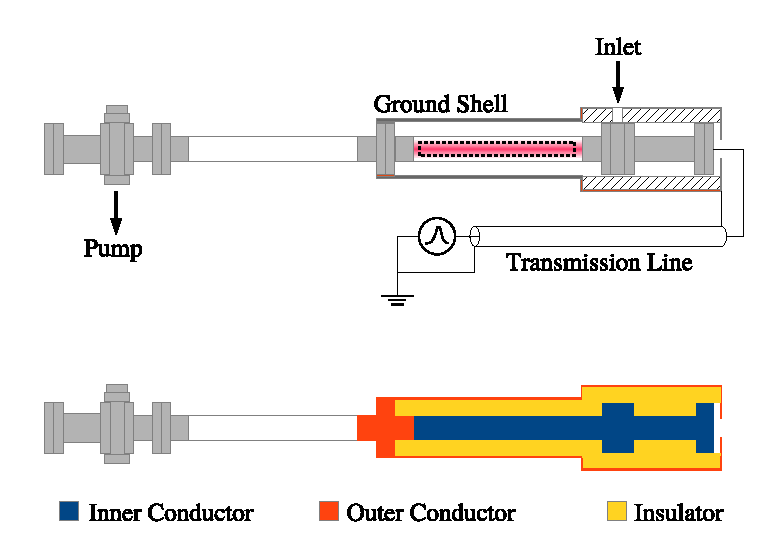
\includegraphics{./chapters/experiment/figures/appschem.eps}
  \caption{Two illustrations of the \acs{rpnd} apparatus. The upper version is
    an annotated sketch of the device, and the bottom version simplifies the
    geometry into its three electrical components.}
  \label{fig:appschem}
\end{figure}
Following from right to left, the inner conductor was composed of a vacuum
window, a Conflat nipple, a double-sided flange tapped for an \textsc{npt}
connection, and the discharge tube containing the plasma.

The tube was composed of borosilicate glass with 2.75 in Conflat flanges on both
ends. The plasma was generated inside the glass tube after it had been evacuated
of air and filled with the desired pressure of helium. The tube had an inner
diameter of 3.3 cm, an outer diameter of 4.0 cm, and a length of 22.9 cm. The
overall length of the tube with the flanges was 30 cm. In the figure shown here,
the right electrode served as the anode, and the left electrode was the cathode.

The dielectric surrounding the inner conductor was composed of several
components. The vacuum window, nipple, double-sided flange, and anode were
separated from the outer conductor by an air gap and a polytetrafluoroethylene
(\acs{ptfe}) tube (hatched in the figure), 20 cm in length with an inner
diameter of about 7.5 cm, and an outer diameter of 10 cm. The plasma portion of
the inner conductor was separated from the outer conductor by an air gap and the
glass tube.

The cathode connected to the outer conductor and served as part of the current
return path. Attached to the cathode was an aluminum tube (referred to as the
ground shell), held in place by a acetyl resin shaft collar and copper
shim.\footnote{While all of the aluminum tube is nominally at ground, it is
likely that it would float to a finite voltage with each pulse.} Radial optical
access to the discharge was provided by two slots milled into the ground shell.
The slots were positioned on opposite sides of the shell and were 3.8 by 25.4 cm
in length. The tube itself was 30 cm in length.

At the end nearest to the anode, the aluminum tube was affixed to a copper
sheet, 10 cm square, with conductive copper tape. A 5 cm diameter hole was cut
into the copper sheet to allow the discharge tube to pass through it. The sheet
was secured to the \acs{ptfe} tube by nylon screws. Surrounding the \acs{ptfe}
tube was a second shell, made of copper sheet. This was connected to the
aluminum tube by a braided copper strap. The right end of the \acs{ptfe} tube
was covered by a second copper sheet, 10 cm square. The sheet was secured to the
\acs{ptfe} tube by nylon screws and in electrical contact with the copper shell.
In the center of the copper sheet was a HN bulkhead adapter for connection to
the transmission line. The inner conductor of the bulkhead adapter was connected
by a straight run of 5 cm of silicone-coated wire to the vacuum window flange.

The voltage pulse was generated by a \acs{fid} power supply, supplied by
\textsc{anvs}, Inc. (model \smaller{PT510NM}). The amplitude of each pulse was
fixed at 6.4 kV with a repetition rate of 1.0 kHz. Each pulse had a fixed width
of 25 ns, with a 10\%-90\% rise time of approximately 4 ns and was roughly
Gaussian in shape. From a practical standpoint, the high impedance prior to
breakdown should effectively double the peak voltage at the anode. A
\textsc{srs} \smaller{DG645} delay generator was used to trigger the power
supply output for all experiments and provided a reference time base for all
measurements.

Preliminary experiments revealed multiple reflections between the power supply
and the anode. A 13.7 m transmission line, made of RG213 coaxial cable, was used
to isolate the reflections so that the effect of individual pulses could be
examined. The calculated delay of the transmission line was 69.2 ns, for a total
separation time between the pulse and the reflection of 138.4 ns. The calculated
delay was found to be a close match in the measured delay.

The gas inlet connection was made through the double-sided flange via a 1/8"
\textsc{npt} hole. A 1/4" polyethylene tube was attached to the \textsc{npt}
connection via a \textsc{npt} to 1/4" Swagelok adapater. The tube was then
connected to a source of ultra-high purity (99.999\%) helium. Throughout the
experiment, the helium flow rate was fixed at 25.0 sccm with a digital flow
controller, regardless of the operating pressure.

The discharge apparatus was pumped down by a oil-based roughing pump with an
upstream zeolite trap. The pump was connected to the discharge tube by a second
glass tube, intended to electrically isolate it from the cathode. The base
pressure of the system was approximately 15 mTorr. The leak rate was measured
several times by evacuating the apparatus and then sealing it from the pump with
a bellows valve. The leak rate was found to be $2.0\times 10^{-3}$ sccm. Given a
constant flow rate of 25.0 sccm, the fractional impurity can be conservatively
estimated to be 80 ppm.

A \textsc{mks} \smaller{PDR-C-2C} power supply and readout, and two capacitance
manometers were used to measure the pressure. One manometer had a full scale
range of 10 Torr, while the other had a range of 100 Torr. The desired pressure
was obtained by sealing the system from the pump with the bellows valve. Two
bypass pump lines, fitted with needle valves, were then used to adjust pumping
speed and system pressure.

The assembled discharge apparatus can be seen in figure~\ref{fig:appphoto}.
\begin{figure}
  \centering
  \setlength\fboxsep{0pt}
  \setlength\fboxrule{1.0pt}
  \fbox{\includegraphics{./chapters/experiment/figures/appphoto.jpg}}
  \caption{Photograph of the discharge apparatus.}
  \label{fig:appphoto}
\end{figure}
The \acs{rpnd} apparatus was supported two 1.5 in mounting posts with angle
brackets. The mounting posts attached to a 4 ft by 2.5 ft optical breadboard,
supported by urethane shock absorbers, and a rigid frame. The roughing pump was
attached to the apparatus with flanged bellows in order to reduce vibrations. 

All electrical measurements were made with a LeCroy \smaller{6100A} WaveRunner
oscilloscope which had a bandwidth of 1.0 GHz. Electrical connections to the
oscilloscope were made with \smaller{RG 50/U} coaxial cable and standard
\textsc{bnc} connectors, terminated at 50 $\Omega$ unless otherwise noted. The
voltage of the pulses was monitored from $1:1000$ divider built into the power
supply. The current was measured from a current shunt located in a break of the
outer conductor of the transmission line. The current shunt was composed of 9,
low inductance, $1.0 \Omega$ resistors connected in parallel.
Figure~\ref{fig:bcs}
\begin{figure}
  \centering
  \setlength\fboxsep{0pt}
  \setlength\fboxrule{1.0pt}
  \fbox{\includegraphics{./chapters/experiment/figures/bcs.jpg}}
  \caption{Photograph of the back-current shunt used to measure the current
  characteristics of the \acs{rpnd}.}
  \label{fig:bcs}
\end{figure}

Data were retrieved from the oscilloscope with a desktop computer via the
\textsc{gpib} interface. Instrument control, data acquisition, and data storage
were all managed by a LabView program. Analog input and output was handled with
the auxiliary input and output ports of a \textsc{srs} \smaller{SR850 DSP}
lock-in amplifier.

\section{Field Calculations}

The electric field characteristics of the discharge system was analyzed using a
two-dimensional, electrostatic solver, Ansoft Maxwell 9. Figure~\ref{fig:fields}
\begin{figure}
  \centering
  \includegraphics{./chapters/experiment/figures/fields.jpg}
  \caption{Heat map and vector plot of the electric field in the \acs{rpnd}
  discharge apparatus.}
  \label{fig:fields}
\end{figure}
is a heat map on a logarithmic scale, of the electric field magnitude, with
overlaid electric field vectors (in magenta). The electric field varies
significantly over the length of the discharge apparatus, with a peak near the
axial location of the glass tube followed by a monotonic decline. These
characteristics are a large departure from simple case of two parallel
electrodes in which the field is uniform throughout. This can be attributed to
the presence of the external ground shield. Though this does complicate the
field characteristics, the proximity of the ground results in a much higher
electric field than would otherwise be achievable.

While the off-axis field lines all feature notable radial components,
particularly close to the anode the center line does not.
Figure~\ref{fig:centere}
\begin{figure}
  \centering
  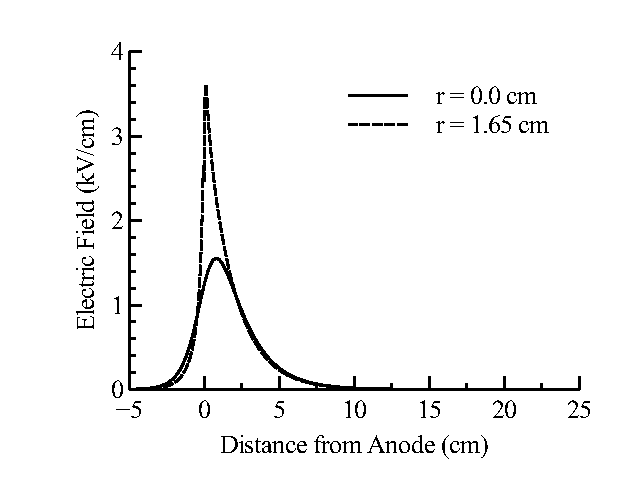
\includegraphics{./chapters/experiment/figures/centere.eps}
  \caption{The magnitude of the electric field along the center and outside of
  the discharge apparatus.}
  \label{fig:centere}
\end{figure}
is a plot of the magnitude of the electric field along the central axis of the
discharge apparatus and the outside, adjacent to the glass tube. The location of
the anode is defined as the location of the glass-to-metal seal. The field close
to the triple point at the seal is the highest at approximately 3.5 kV/cm, while
the field along the axis peaks at about 1.5 kV/cm. At a distance of 2 cm from
the anode, the electric field magnitude is roughly the same regardless of the
radial coordinate. At the measurement locations of 3.83, 11.45, and 19.07 cm,
the vacuum electric field was $4.8 \times 10^5$, 750, and 11 V/m respectively. 

\section{Operating Procedures}

One of two operating procedures was selected depending on how recently the
plasma had last been turned on. If it had been greater than one hour, a full
startup procedure was used. Otherwise, an abbreviated process was used. 

In order to obtain consistent discharge characteristics, it was necessary to
develop two sets of operating procedures for the \acs{rpnd}. In the case that
the discharge had not been operated for over an hour, the roughing pump was
turned on and the primary pump path valve was opened as was the first shutoff
valve upstream of the discharge chamber, seen in figure~\ref{fig:pump}.
\begin{figure}
  \centering
  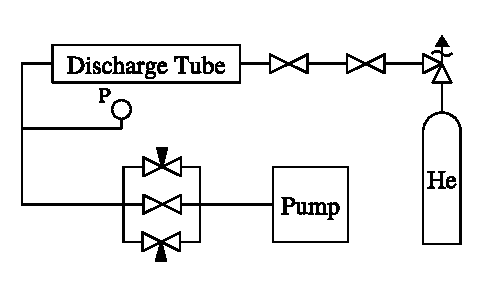
\includegraphics{./chapters/experiment/figures/pump.eps}
  \caption{Simplified diagram of the gas flow path and pumping system.}
  \label{fig:pump}
\end{figure}
The system was then allowed to pump down to its base pressure. Afterward the
final shutoff valve upstream of the pump path was opened and the system was
again allowed to reach base pressure. At this point the helium flow was turned
on and set to 25.0 sccm. The primary pump path was then closed and the needle
valve bypasses were used to adjust the system pressure to 3.0 Torr.

Next, the delay generator was turned on and the output for triggering the power
supply was activated. Then, the \acs{fid} power supply was then turned on. This
would produce an easily visible plasma within the discharge tube. The system was
allowed to operate at this condition for one hour in order to remove potential
contamination on the walls and electrodes. At the end of this period, the pulse
voltage waveform was checked to ensure that it was consistent with previous
waveforms. Once this was confirmed, the pressure was adjusted to the desired
operating condition.

The plasma was shutdown by first shutting off the power supply, followed by the
delay generator. Then, the helium flow was shut off, and the primary pump path
was opened. The system was allowed to come to base pressure before the two
upstream shutoff valves were closed, after which the primary pump path was
closed. The roughing pump was then shut off.

In the cases that the plasma had been operated within the last hour, it was
possible to use an abbreviated startup procedure. This process was fundamentally
the same as the previous one, however the plasma only required five minutes to
reach a steady state. This was verified with multiple measurements of the
current and voltage characteristics as well as the plasma emissions. At times
prior to this five minute equilibration period, the reflected pulse energy was
noticeably higher, and the delay between the trigger pulse and the output pulse
was variable.

\section{Electrical Characteristics}

The general voltage waveform of the \acs{rpnd} showed a number of
characteristics. Figure~\ref{fig:waveform}
\begin{figure}
  \centering
  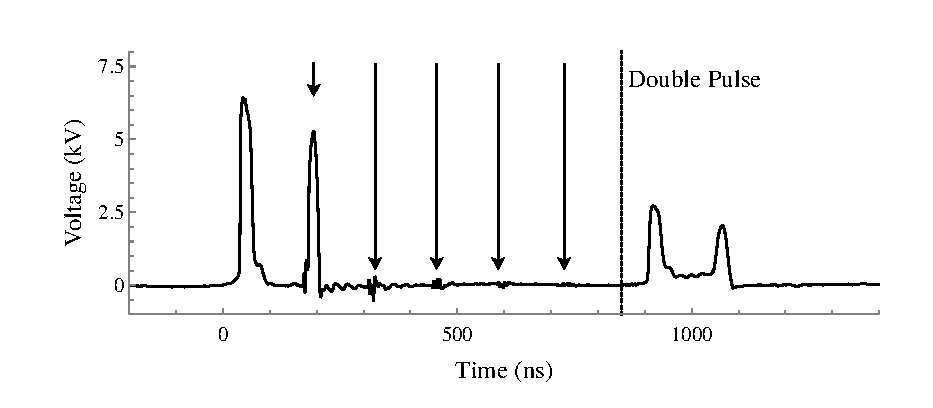
\includegraphics{./chapters/experiment/figures/waveform.eps}
  \caption{Typical voltage waveform of the \acs{rpnd}. Arrows indicate
    reflections back to the power supply. The dotted line delineates the time at
    which the power supply begins to exhibit double pulsing.}
  \label{fig:waveform}
\end{figure}
is a plot of a typical voltage waveform of the \acs{rpnd}. It begins with an
incident pulse with a small foot at $t = 0.0$. This followed by a reflected
pulse 138 ns afterward. The reflected pulse is somewhat attenuated, proportional
to the energy deposited in the plasma. Additional reflections are visible at
integer multiples of 138 ns, however they are highly attenuated. This suggests
that after the first pulse initiates the discharge, energy is much more easily
coupled into the volume. An additional pulse appears after about 800 ns. This is
believed to be a peculiarity of the power supply. For the most part, analysis of
the \acs{rpnd} will focus on the first 138 ns in order to isolate the effects of
a single pulse.

The independent variable for most operating conditions was the pressure of the
system. The properties of the \acs{rpnd} were examined at: 0.3, 0.5, 1.0, 2.0,
3.0, 4.0, 8.0, and 16.0 Torr. The appearance of the plasma varied with the
pressure in a continuous fashion, however it was apparent that there were three
regimes of operation.

At the low pressures, 0.3 and 0.5, it was difficult to initiate the discharge.
Often, it would be necessary to increase the pressure to initiate the discharge,
and then reduce the pressure to the desired conditions. The plasma appeared dim
and relatively constricted to the central axis of the discharge tube, with a
radial extent of approximately 1 cm. Accompanying these presures was a large
degree of electronic noise. This manifested in the voltage and current
waveforms, seen in figure~\ref{fig:waveforms},
\begin{figure}
  \centering
  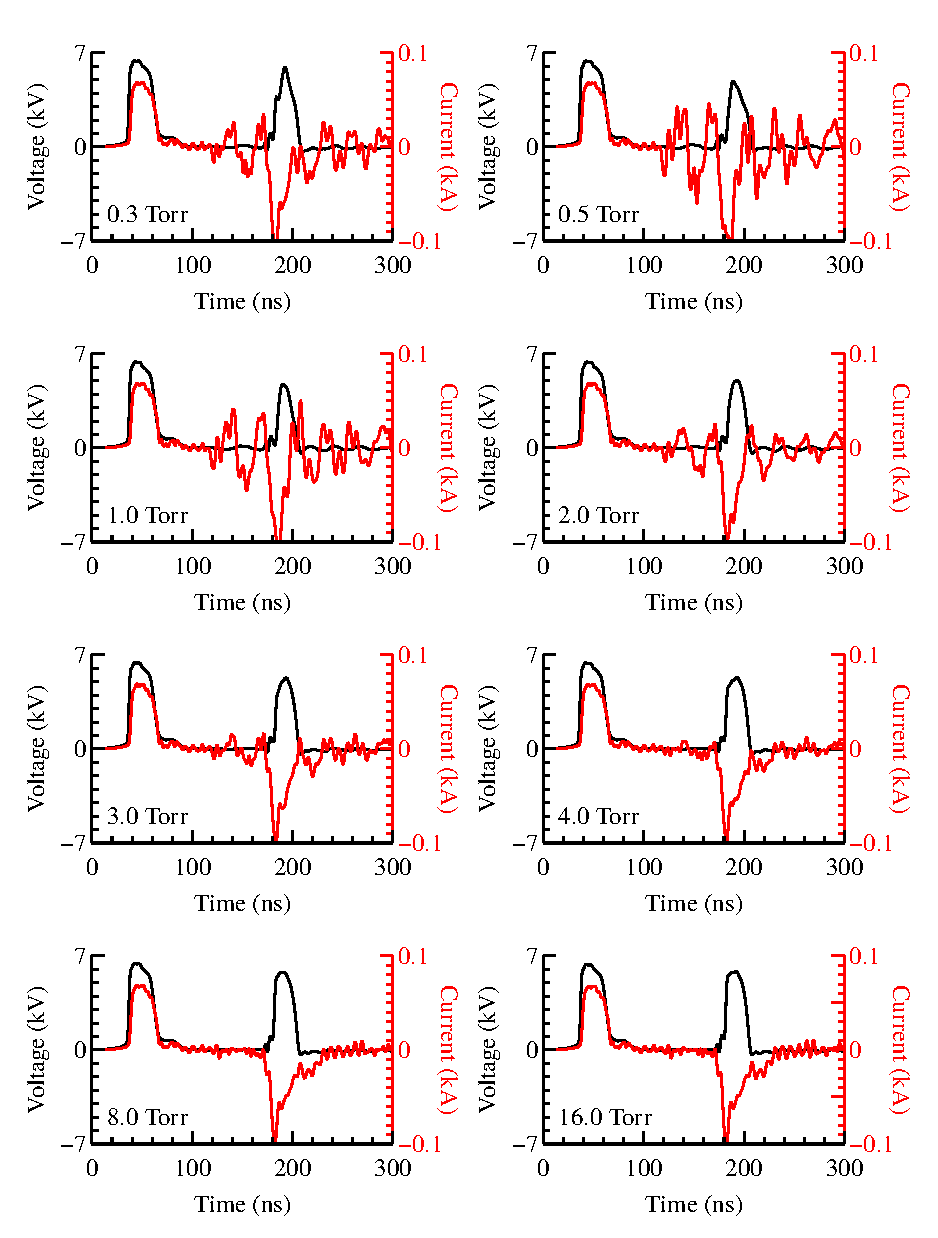
\includegraphics{./chapters/experiment/figures/waveforms.eps}
  \caption{High resolution views of the voltage and current waveforms for the
  first incident and reflected pulse, at each of the operating pressures.}
  \label{fig:waveforms}
\end{figure}
as well as a number of equipment malfunctions.

As the pressure was increased (from 1.0-4.0 Torr), the electrical noise began to
subside. The waveforms in figure~\ref{fig:waveforms} show significant reductions
in the ringing that was particularly prominent in the current waveforms. In
addition, the visual extent of the plasma increased substantially to the point
where it could be considered volume-filling. The plasma also increased its axial
extent as well, eventually reaching well past the cathode/ground. This was
despite attempts to isolate this portion of the apparatus from the plasma. It is
possible to attribute this to the relatively large surface area of the anode in
comparison to the cathode. If a sufficiently high electron current is being
drawn from the cathode, space charge could begin to limit further current
extraction.

However, the plasma receded back to the intended cathode structure at the higher
operating pressures, 8.0 and 16.0 Torr. This was accompanied by a decrease in
the apparent brightness of the plasma to levels similar to that of the low
pressure conditions. In contrast, the plasma appeared to remain volume-filling.
While discharge initiation was difficult at the higher pressures, it was not
accompanied by the electrical noise observed at lower pressures.

\section{Energy Coupling}

The product of the voltage and current waveforms as seen in
figure~\ref{fig:waveforms} gives the power deposited in the plasma as a function
of time. Subsequently, the power integrated over time gives the total energy
deposited in the plasma. However, this approach is somewhat complicated several
features of the \acs{rpnd}. As previously mentioned, the pulses produced by the
power supply are not completely absorbed by the plasma. Therefore, the
integration must be carried out over both the incident and the reflected pulse.
Additionally, there is the concern that the oscillations in the current
measurements could introduce fluctuations in the calculated energy deposition.
However, the small voltage signal limits the error introduced by these
fluctuations to less than 1\%.

Figure~\ref{fig:energies}
\begin{figure}
  \centering
  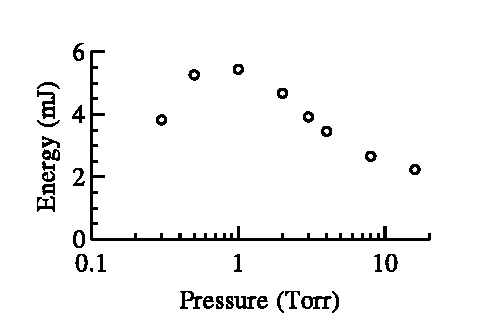
\includegraphics{./chapters/experiment/figures/energies.eps}
  \caption{Plot of the energy coupled into the plasma with the first pulse as
  a function of pressure.}
  \label{fig:energies}
\end{figure}
gives the total energy deposited for the first pulse at each of the operating
conditions. The energy coupled to the plasma peaks at an energy of 5.5 mJ at a
pressure of 1.0 Torr, after which it slowly decreases. This peak in the coupled
energy is coincident with the peak brightness of the plasma. Together, these
suggest that the density of excited states will be optimized at intermediate
pressures. 

Though there appear to be no direct comparisons available in the literature,
several papers report on energy coupling for similar systems. Macheret,
Schneider, and Murray studied a parallel plate \acs{rpnd} in air, at 1-10 Torr
and reported a total energy deposition of 0.30-0.36 mJ, increasing with pressure
\cite{Macheret2006}. Nishihara et al.\ recorded values of 1-2 mJ in a nitrogen
\acs{rpnd} \cite{Nishihara2006}. Pancheshnyi et al., in the study of an
air-propane mixture at 750 Torr, found that each pulse deposited about 1.9 mJ of
energy.

From an applications standpoint, potential existence of a condition which
optimizes the production of excited states is an interesting one. From a
physical standpoint, the growth and decline of energy deposition is with power
is compelling as it suggests two or more competing processes. Though this kind
of competition is reminiscent of Paschen's law, the duration of the pulse is too
short for appreciable ion drift (about 3 mm for the maximum field from the
electrostatic simulations), therefore secondary electron emission is not
important. These observations provide additional impetus for a closer
examination of the \acs{rpnd} properties, particularly the excited states.


  \chapter{Metastable Measurements}\label{chp:metastables}
    As was noted in chapter~\ref{chp:introduction}, measurements of the \acs{rpnd}
been mostly limited to the afterglow plasma or time-integrated quantites.
Electric field measurements, either with capacitive probes or nonlinear
wave-mixing, thus far provide the only detail of the \acs{rpnd} during its
development. Though the electric field can be used to estimate electron
densities and reaction rates in the plasma, this requires a number of additional
assumptions.

As a result, there is a lack of reliable information on the particle properties
of the \acs{rpnd} during its development. That said, such information is
essential to confirming the present understanding of how these discharges
develop, optimizing them for specific applications, and providing important
benchmarks for numerical simulations. Therefore, a clear need exists for direct
measurements of the \acs{rpnd} particle properties.

Unfortunately, these measurements present a significant challenge for most
traditional plasma diagnostics. In most situations, the obvious choice would be
the Langmuir probe for its simplicity and ease of implementation. However, the
fast variations in the plasma potential, slow response of the ion, and high
collisionality all preclude this approach \cite{Lieberman2005}. Furthermore, any
physical probe would act as a significant perturbation in the system.

The logical alternative to physical probes is the use of optical diagnostics,
however these have their own associated difficulties. Electrons cannot be
studied by their emissions because, with the exception of bremsstrahlung, they
do not emit light. This leaves the light emitted from excited atoms. Atomic
emission spectroscopy can be used to measure many different plasma quantities,
from electron density, to local electric field strength. Unfortunately,
spontaneous emission can be a slow process compared to the development of the
\acs{rpnd}. For example, the fastest neutral helium transition in visible
wavelengths (3$^3$D$_3$-2$^3$P$_2^\cdot$) has a radiative life of 14 ns
\cite{Ralchenko2011}.

This suggests that instead of waiting for spontaneous emission to occur, it may
be better to use some form of active spectroscopy. Though the added complexity
of a well-characterized light source is undesirable, it adds several interesting
possibilities. For example, Thomson scattering provides a means for direct
interaction with electrons. In addition, it has a high spatial and temporal
resolution and is able to measure the electron density and temperature
simultaneously \cite{VanGessel2012}. However, the electron density limit of
$5\times10^{12}$ cm$^{-3}$ is too low for use with the \acs{rpnd} which may have
electron densities well below this \cite{Pai2009}.

With the ability to directly interact with electrons, the next alternative is to
target one of the excited states of helium. The lowest such state, the triplet
metastable (2$^3$S), resides at 19.82 eV. This is a relatively large energy gap
for an atom and indicates that virtually no such states should exist at room
temperature. The triplet metastable (and all higher-energy states in helium)
will be populated exclusively by energetic electrons. Therefore, a measurement
of the triplet metastable level is a useful indicator of the degree of helium
excitation as the \acs{rpnd} develops, and could potentially be used to infer
some properties of the electron population.

Perhaps the most straightforward approach to a measurement of the triplet
metastable density is with absorption spectroscopy. This approach has a long
history in the study of metastables in gas discharges, going back at least six
decades \cite{Phelps1953}. At its most basic, the technique involves
illuminating a plasma with light matching a transition between the metastable,
and some upper level and measuring the amount of light transmitted. The amount
of light transmitted is proportional to the metastable density integrated along
the path of the light traversing the plasma. The bandwidth of this measurement
is only limited by the time required for the light to pass through the plasma.

\section{Setup}

Traditionally, the light used in absorption spectroscopy has been supplied by
discharge tubes with the same gas as the system under study. Though
straightforward, this approach is limited by the luminosity of the discharge
tube, and the fact that the emitted radiation is isotropic. More recently,
Millard et al. noted that diode lasers provide a greatly improved light source
that provides simple spatial selectivity, at intensities which can easily exceed
the saturation limit \cite{Millard1998}.

As with the study by Millard et al., the decision was made to study the
transition from the triplet metastable to the 2$^3$P$^\mathrm{o}_{0,1,2}$ (at
approximately 1083 nm). This was done for several reasons. For one, the closest
helium transition is over 7 nm away, making it relatively isolated. In addition,
the different levels or values of $J$ are all within the tuning range of a
single diode. As each level has a different degeneracy, $g$, the strength of
absorption varies depending on the selected level. Thus, the absorption strength
can be increased for low densities, or decreased at high densities, improving
the dynamic range of the diagnostic.

The laser used was a distribute feedback laser diode, produced by Toptica, model
LD-1083-0070-DFB-1. The specified linewidth of the laser was 3 MHz, well below
the natural linewidth of the transition, 10.2 MHz. This situation can be
exploited to directly measure the gas temperature of the system, as will be seen
in the next section. The diode was rated for a total output power of 70 mW, with
a beam size of 1 mm by 3 mm and a vertical polarization. The diode was housed in
a Toptica DL DFB housing which incorporated the collimating optics. A Toptica
DCC 110 was used to provide current control for the diode laser, and a Toptica
DTC 110 was used to control the thermoelectric cooler for the diode.

The layout in figure~\ref{fig:laser}
\begin{figure}
  \centering
  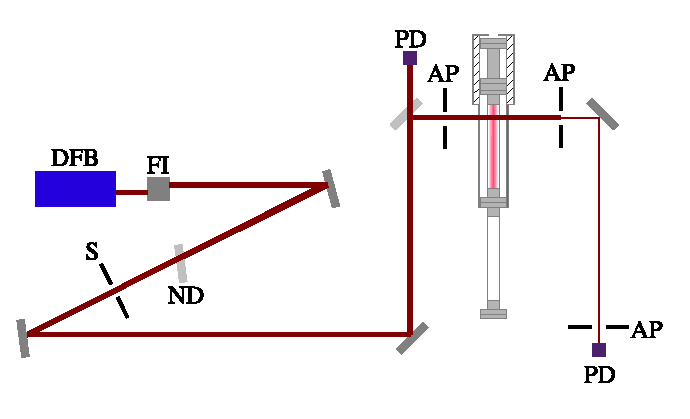
\includegraphics{./chapters/metastables/figures/laser.eps}
  \caption{Optical beam path of the laser in the absorption spectroscopy
  experiment. DFB - Distributed feedback laser diode; FI - Faraday isolator; ND -
  neutral density filter; S - shutter; PD - photodiode; AP - aperture.}
  \label{fig:laser}
\end{figure}
reflects the optical beam path used in the absorption experiment. The laser
light is produced by the distributed feedback laser diode (DFB). It then enters
a Electro-Optics Technology, Inc. Faraday isolator (FI) which prevents
back-reflections from entering the diode. Without the isolator in place, such
back-reflections can cause mode-hopping, resulting in unreliable tuning. The
laser intensity is then reduced by a neutral density filter (ND). Afterward, the
laser passes through a Vincent Associates electronic shutter (S). Then, the beam
is split by a Thorlabs BSF10-C beam sampler at a 45$^\circ$ angle. This reduced
the laser intensity below the saturation intensity (0.45 mW/cm$^2$) of the
transition. Collimation to a 1 mm circle, and alignment were provided by two
apertures (AP) on both sides of the discharge apparatus. The beam exiting the
apparatus was then sent through a final aperture to spatially filter plasma
emissions before being a Thorlabs F240SMA-780 collimation package was used to
couple the light into an optical fiber.

Behind the beam sampler was a Thorlabs DET300 germanium photodiode. The signal
from this photodiode was terminated at 1 M$\Omega$ and used to monitor the beam.
The opposite end of the optical fiber was affixed to a Thorlabs DET410 InGaAs
photodiode. The photodiode signal was amplified by a Femto HVA-200M-40-B voltage
amplifier before being sent to the oscilloscope. The time resolution of the
metastable measurements was determined by the InGaAs photodiode which had a
specified rise time of 5 ns.

In order to measure the absorption of the laser, it was first necessary to tune
the laser to the correct wavelength. This matter was complicated by the lack of
a wavemeter with sufficient precision and accuracy. As a result, a signal
generator was used to sweep the laser current so as to cover a frequency range
of 40 GHz. The temperature of the diode was then slowly adjusted until
absorption peaks corresponding to the 2$^3$S$_1$-2$^3$P$_{0,1,2}^\mathrm{o}$
transition were observed. The conversion between diode and wavelength was
measured with a CVI Melles Griot ET-25.4-10.00-30, solid dielectric etalon. It
was found that a temperature of 36$^\circ$ C and a current of 63 mA produced
resulted in an output wavelength of approximately 1082.9 nm.

As described in chapter~\ref{chp:experiment}, data acquisition was handled by a
LabView program, connected to the oscilloscope by GPIB\@. The auxiliary outputs of
the SRS SR850 lock-in amplifier were used to adjust the diode laser current (via
the DCC 110 module), and to trigger the electronic shutter. One of the auxiliary
inputs of the lock-in amplifier was used to read out the pressure from the
pressure controller.

Data were acquired for a range of pressure 0.3-16.0 Torr, and at three axial
locations: 5.08, 12.7, and 20.32 cm, relative to the glass-metal seal of the
anode. In reference to their location relative to the gas inlet these will be
referred to as the `upstream', `midstream', and `downstream' locations,
respectively. For each combination of location and pressure, absorption spectra
were measured over $\pm3.85$ GHz relative to the nominal transition frequency of
the 2$^3$S$_1$-2$^3$P$_0^\mathrm{o}$ transition at intervals of 154 MHz. The
absorption spectra were measured for time domains of $-300$-$1700$ ns relative
to the voltage pulse. Additional measurements were made at the midstream
position of the metastable densities from $-88$-$712$ $\mu$s in order to
investigate the loss mechanisms of the metastables.

The broadband electronic noise emitted by the fast pulses was a persistent issue
and presented one the greatest challenges to measurements during the \acs{rpnd}
development. As described above, the InGaAs photodiode was removed from the
immediate area surrounding the discharge by an optical fiber. The optical fiber
was routed through a small opening in a grounded metal box where both the
photodiode and the voltage amplifier resided. In addition, the DC power supply
of the voltage amplifier was connected to an outlet on a Tripp-lite Isobar
intended to provide additional isolation. The photodiode was connected directly
to the input terminal of the amplifier, while the amplifier was connected to a
BNC bulkhead adapter by a 10 cm length of RG 50/U. The final connection to the
oscilloscope was made by an additional 10 cm length of RG 50/U, running from the
BNC bulkhead connection.

Figure~\ref{fig:transmitted}
\begin{figure}
  \centering
  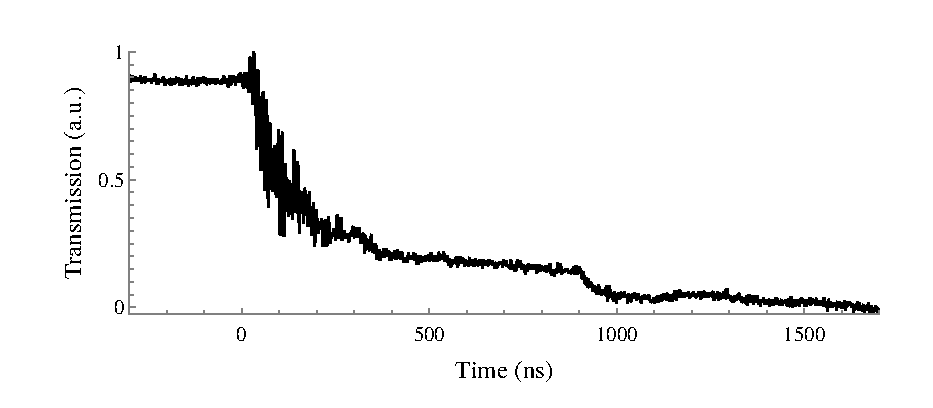
\includegraphics{./chapters/metastables/figures/transmitted.eps}
  \caption{Measurement of the transmitted laser light at the nominal transition
  wavelength at 4.0 Torr of helium.}
  \label{fig:transmitted}
\end{figure}
shows the transmission signal measured at the nominal transition wavelength for
a \acs{rpnd} in 4.0 Torr of helium. The signal is the average of 200 independent
pulses, further sampling had no appreciable effect on the waveform. As can be
seen, despite the efforts to limit the electrical interference, there is still a
substantial amount of noise present in the transmission signal. This is most
noticeable in the large ringing which occurs for the first 200 ns after the
voltage pulse. Without any kind of compensation, it would be impossible to
obtain reliable measurements of the transmission signal

\section{Absorption Analysis}

The noise produced by the \acs{rpnd} was relatively consistent between pulses
and over the duration of each experiment. As a result, it was possible to
correct for the electrical noise, as well as any spontaneous plasma emissions,
by measuring the signal from the photodiode in the absence of the laser. The
acquisition process proceeded as follows:
\begin{enumerate}
  \item Set desired laser wavelength.
  \item Wait 5 s for laser output to settle.
  \item Acquire 200 waveforms from photodiode.
  \item Close shutter.
  \item Acquire 200 waveforms from photodiode.
  \item Repeat
\end{enumerate}
The second set of waveforms was then subtracted from the first in the
post-processing stage. The effect of this subtraction can be seen in
figure~\ref{fig:contours}
\begin{figure}
  \centering
  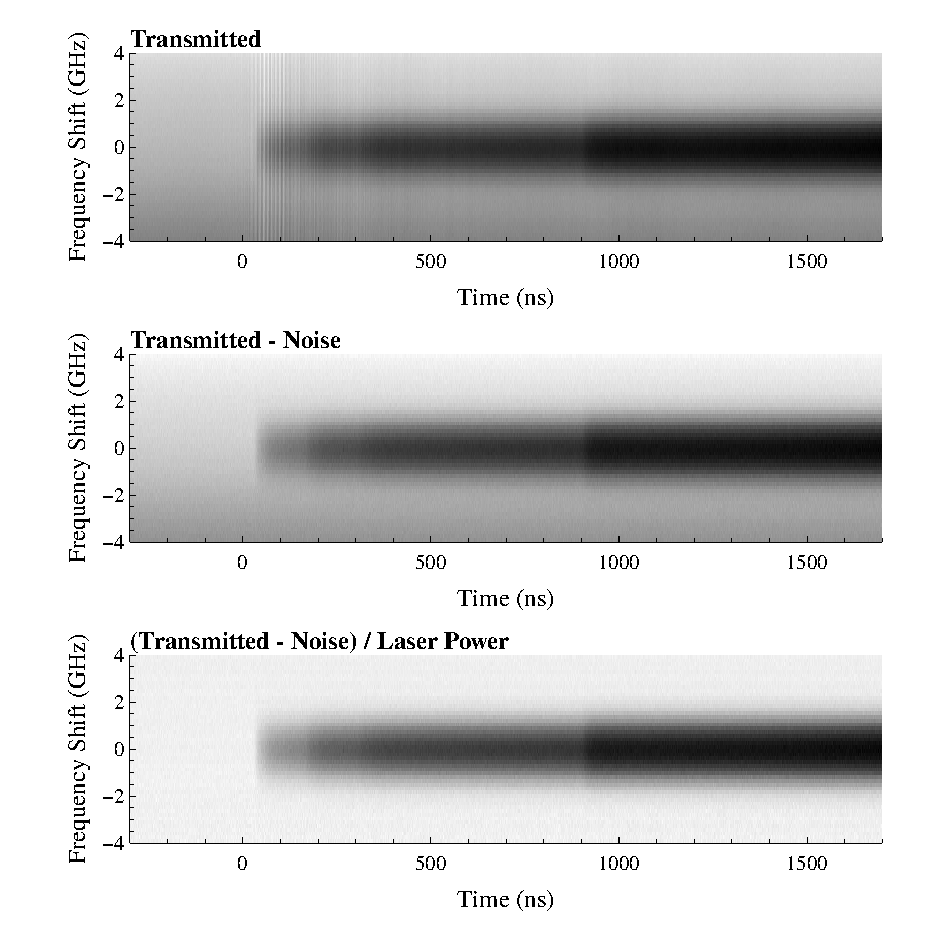
\includegraphics{./chapters/metastables/figures/contours.eps}
  \caption{Heatmaps of the transmitted laser signal for the 4.0 Torr condition at 
  various stages of post-processing.}
  \label{fig:contours}
\end{figure}
where the top heatmap shows the initial set of acquisitions with the laser on,
and the middle heatmap shows the transmitted signal with the noise subtracted.

As the laser diode current was changed in order to scan the wavelength across
the transition, the output power also changed by a small but significant amount.
The produces the gradient-like appearance of the top two plots in
figure~\ref{fig:contours}. In order to obtain a measurement of the unattenuated
laser power, the above acquisition procedure was repeated with the plasma off
for each operating condition. This made it possible to correct for the varying
laser power and to produce properly scaled transmission spectra.

These transmission spectra were then analyzed using a transmission model based
on the absorption cross sections described in chapter~\ref{chp:theory}. In a
one-dimensional system, the change in intensity of an incident photon field
(below the saturation limit), can be expressed as
\begin{equation}
  \frac{dI(x, \omega)}{dx} = -\sigma(\omega) N(x) I(x, \omega)
\end{equation}
where $I$ is the intensity of the photon field as a function of distance $x$,
$\omega$ is the frequency of the photons, $N$ is the density of the interacting
species, and $\sigma$ is the interaction cross section. This equation has the
simple solution,
\begin{equation}
  T(\omega) = \frac{I(x, \omega)}{I_0(\omega)}
            = \exp\left[-\sigma(\omega) \int_0^x N(x') dx'\right],
  \label{eq:transmitted}
\end{equation}
where $T$ is the transmitted intensity fraction, and $I_0$ is the initial
intensity of the photon field. The absorption can be trivially obtained from the
equation $A(\omega) = 1 - T(\omega)$.

For the purpose of analyzing the absorption, a quantity called the
line-integrated density will be defined. This is simply, $\nint = \int_0^x
N(x')dx'$. Equation~\ref{eq:absorb} can be used to determine the absorption
cross section. However, this requires that a lineshape be specified. If
possible, it is preferable to select either a purely Gaussian or purely
Lorentzian lineshape as the Voigt profile (equation~\ref{eq:voigt}) is
accompanied by a significantly larger computational cost. This can be determined
by a comparison of the relative widths of the different broadening mechanisms.
For a temperature of 300 K and a pressure of 8.0 Torr, it is found that $\dwd =
1.7$ GHz and $\dwa = 0.21$ GHz. Because neither broadening mechanism is
significantly dominant, the choice was made to analyze the data with a Voigt
profile, despite the added computational cost.

Equations~\ref{eq:transmitted},~\ref{eq:absorb}, and~\ref{eq:voigt} can be
combined to form a model equation for the transmitted spectrum. It can be seen
that only two unknowns exist: the gas temperature, $T_g$, and the
line-integrated density, $\nint$. For each time step, this model equation was
matched to the measured spectrum using the Levenburg-Marquardt algorithm
\cite{Marquardt1963} as implemented by the SciPy library \cite{Jones2001}.
During the matching process, it was observed that the diode current for which
absorption was optimized would shift over time. This was assumed to be the
result of small, long-term variations in the diode temperature that were not
adequately compensated for by the temperature control system. This corresponded
to a frequency drift of $\pm60$ MHz between experiments. For each experiment,
this frequency offset was measured for the spectrum with the largest absorption
signal and was then used to correct the analysis of all other spectra.

\section{Results}

The matching algorithm proved robust enough to automatically match the
transmission spectrum at each time step with no user intervention.
Figure~\ref{fig:matching}
\begin{figure}
  \centering
  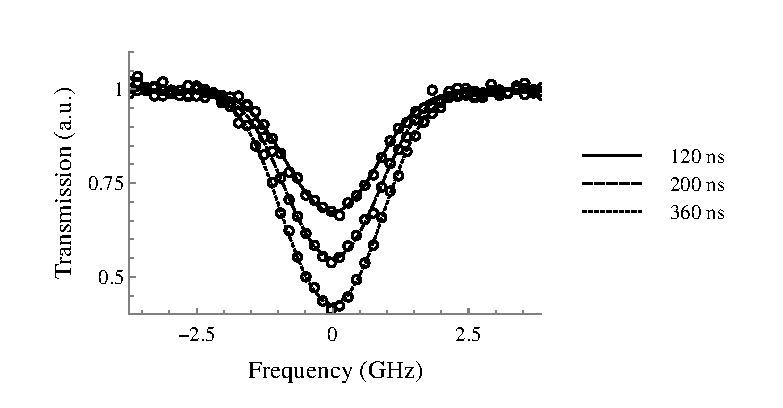
\includegraphics{./chapters/metastables/figures/matching.eps}
  \caption{Comparison of the measured transmission profile (open symbols) and
  the computer-generated matches for at several different times for the 4.0 Torr
  operating condition.}
  \label{fig:matching}
\end{figure}
shows three examples of the measured transmission spectra along with the
computer-generated matches. The measure data far from the peak coincide almost
perfectly with an unabsorbed signal. In addition, the spectrum at 120 ns shows
no evidence of the noise caused by the discharge. The variation in the baseline
transmission signal is approximately 0.02. This sets a minimum line-integrated
detection limit of approximately $3.0 \times 10^{14}$ m$^{-2}$, though the
actual value will depend to some extent on the pressure and temperature.

\subsection{Temperatures}

The temperatures calculated for the metastables from the laser-absorption
spectroscopy are shown in figure~\ref{fig:temperatures}.
\begin{figure}
  \centering
  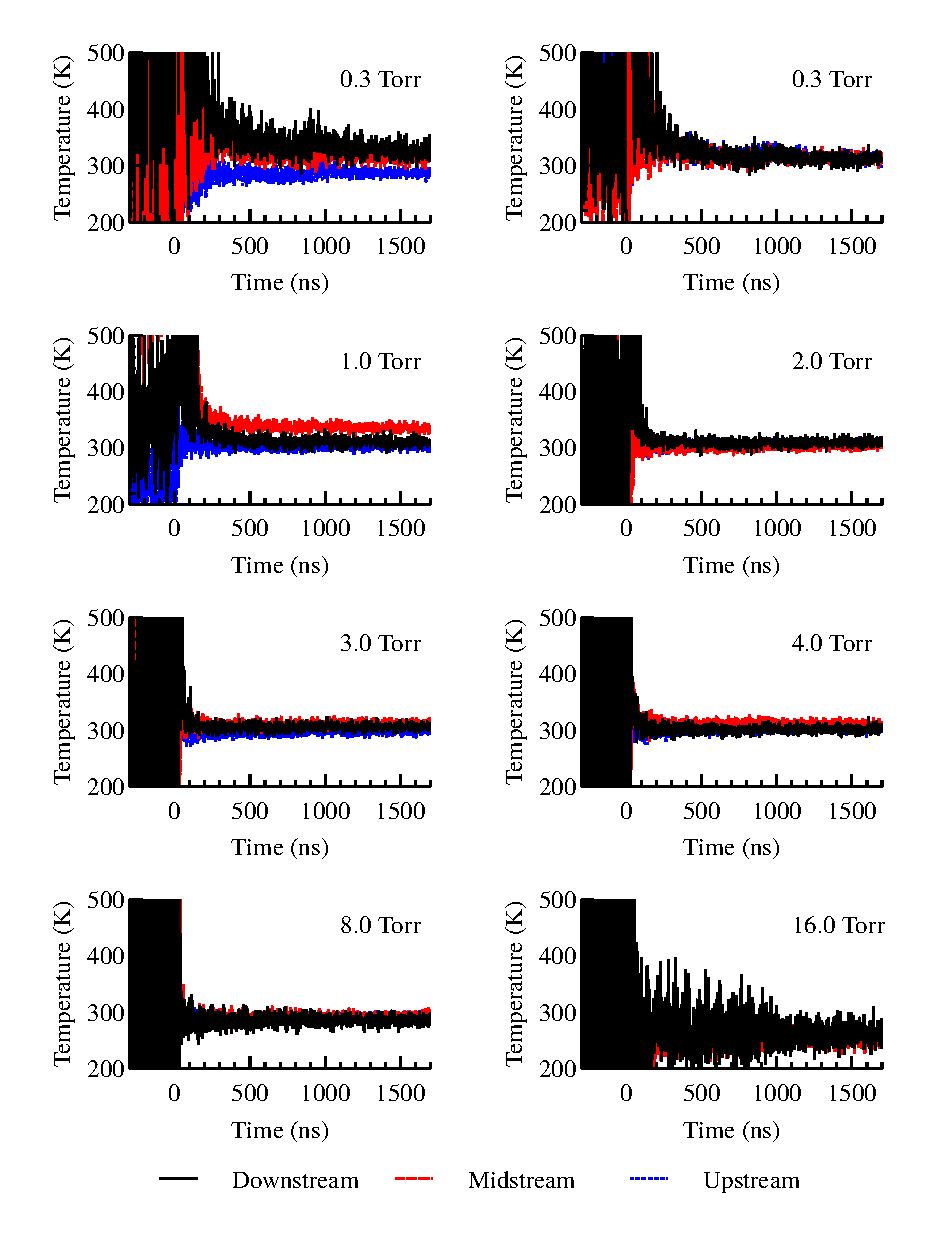
\includegraphics{./chapters/metastables/figures/temperatures.eps}
  \caption{Plot of the gas temperatures at each of the operating
  pressures and each axial location as a function of time.}
  \label{fig:temperatures}
\end{figure}
Prior to the pulse, the temperature estimates are subject to large variations.
This is a result of the low metastable densities which precede the pulse.
Without a substantial metastable population to work with the matching algorithm
has difficult discriminating between a combination of low temperatures and low
densities (a small narrow absorption spectrum) versus high temperatures and high
densities (a very broad absorption spectrum).

It is not possible to precisely calculate the error for the matching process at
each time step, however it is possible to estimate the standard deviation. In
all cases, the estimated standard deviation is less than 10 K by the end of the
measurement period. Based on the covariance estimates, there appear to be no
meaningful trends over the measurement period or between measurement locations.

In order to more clearly compare the temperatures at the different operating
conditions, the results for each location were combined and averaged over the
final 200 ns. This was then plotted with respect to the energy deposition
calculations from chapter~\ref{chp:experiment}, divided by the gas density.
The results are shown in figure~\ref{fig:tvp}.
\begin{figure}
  \centering
  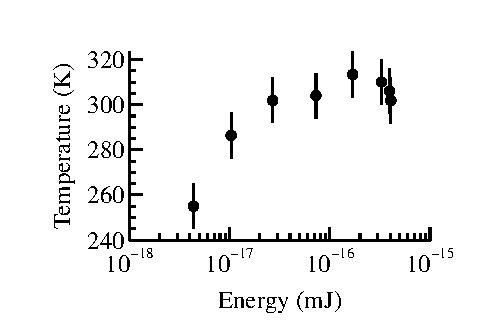
\includegraphics{./chapters/metastables/figures/tvp.eps}
  \caption{Plot of the average gas temperature as a function of deposited
  energy.}
  \label{fig:tvp}
\end{figure}
For the majority of operating conditions, there is little to know statistical
difference between the results and room temperature. The one exceptional
condition is the 16.0 Torr operating condition at 4.33$\times10^{-18}$
mJ/cm$^3$ with a mean temperature of 255 K. As the glass of the discharge tube
as at room temperature for all experimental conditions, this does not appear to
be a reasonable result for the temperature. Examination of the individual
absorption spectra did not reveal any obvious errors in the calculated matches.
However, as will be seen later, the metastables were the least dense at 16.0
Torr. This, coupled with the large variation of the temperatures in
figure~\ref{fig:temperatures} suggest that the standard deviation is potentially
lager than 10 K. Such a situation would explain the unreasonable temperature
obtained for this condition.

The literature provides only a limited number of direct temperature measurements
for similar systems. The most similar work in appears to be that of Walsh et al.
\cite{Walsh2010} in which the temperature of a \acs{rpnd} in helium with a small
admixture of oxygen was measured by optical emissions. The geometry consisted of
two cylindrical steel electrodes separated by 2 mm with a single dielectric
barrier between the two, a gas flow rate of 5 slm, at atmospheric pressure.
Temperatures ranged from 300-340 K, depending on the average power dissipated in
the plasma. Walsh et al. suggest that the observed temperature increase is a
result of Joule heating, that is, heating of the gas as a result of electrons
colliding with neutral particles. As the neutral collision frequency scales
linearly with pressure, this would certainly explain the negligible heating
observed in figure~\ref{fig:tvp}. The presence of a large fraction of a
molecular gas (oxygen) presents another potential heating mechanism when
dissociation occurs, called Franck-Condon heating, and excitation of rotational
and vibrational states which relax to translational energy
\cite{Kiehlbauch2003}.

Other experiments have demonstrated minimal gas heating, as in the case of
plasma bullets \cite{Laroussi2005, Lu2006}, while others have measured final
temperatures ranging from 400-1000 K \cite{Pai2009, Popov2011, Zuzeek2010} (see
appendix~\ref{chp:oes} for detailed study in air). From the available
literature, measurable heating only appeared to coincide with measurements of
\acs{rpnd}s in molecular gases. This emphasizes the importance of the heating
mechanisms mentioned earlier and likely plays a large role in the nonthermal
nature of the atmospheric pressure helium plasmas.

Recent simulations and rate calculations \cite{Takashima2011, Aleksandrov2007}
have provided estimates of the electron temperature in the range of 10-20 eV. As
a result, all of the discharges mentioned are very much nonthermal in nature.
That said, the negligible heating in the helium \acs{rpnd} studied here presents
a significant advantage for many applications, as even the moderate temperature
increases in molecular discharges can threaten material integrity. For example,
most commercial polymers are only rated to 300$^\circ$ C, making them
susceptible to damage without careful thermal management.

\subsection{Line-integrated Densities}

As described in the analysis section, the laser-absorption spectroscopy also
yielded the line-integrated metastable densities. Figure~\ref{fig:metastables}
\begin{figure}
  \centering
  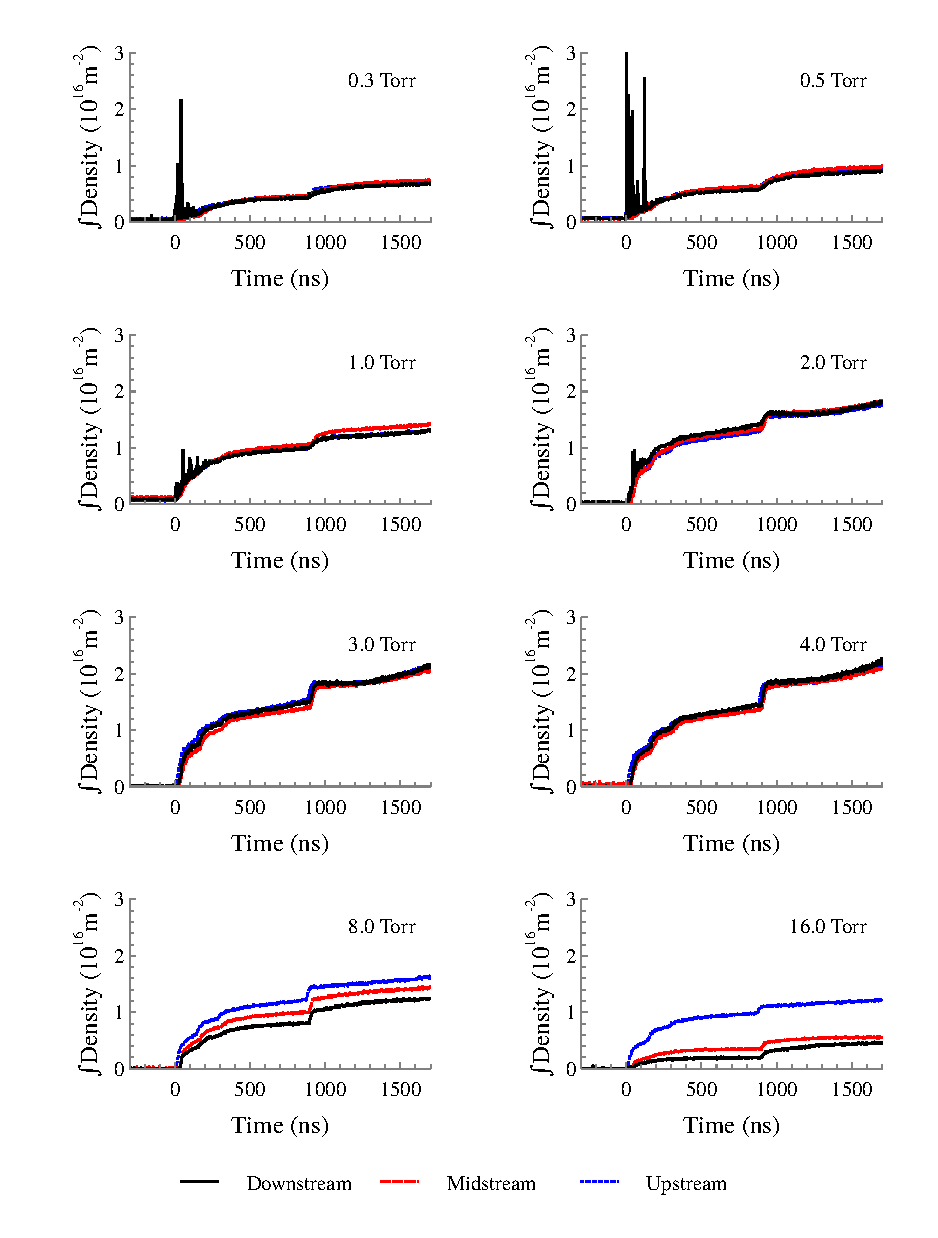
\includegraphics{./chapters/metastables/figures/metastables.eps}
  \caption{Plots of the line-integrated metastable densities at each of
  the operating pressures and each axial location as a function of
  time.}
  \label{fig:metastables}
\end{figure}
features the metastables dynamics for each operating pressure and at each
location. Similar to the temperature measurements, there is a substantial
uncertainty during the pre-pulse period for pressures greater than 1.0 Torr.
However, for 1.0 Torr and below, there are detectable populations of triplet
metastables, around $7\times10^{14}$ m$^{-2}$. These excited atoms are the
remnants of the previous pulses which have not been destroyed. Despite the
efforts made to limit the noise in the signals, there is a significant number of
erroneous data points at pressures below 3.0 Torr in the downstream
measurements. The reason for this is not apparent. The only change was the
position of the mirror directing the transmitted laser light into the fiber
coupler. That is, the position of the photodiode did not change between
measurements. 

The population of the metastable states exhibits several small bursts, in short
succession, after the pulse at about 140 and 270 ns. The timing of these rapid
rises in density correlate to the arrival of pulse reflections. This suggests
that the even after the plasma has formed, additional pulses are still able to
deposit a significant amount of energy in the plasma. In all reported cases, the
final metastable density grew to exceed twice the density after the first pulse.
This appears to contradict the predictions made by the one-dimensional drift
models of Adamovich et al. \cite{Adamovich2009} and Nikandrov et al.
\cite{Nikandrov2008} which stated that little energy is coupled into the plasma
after breakdown occurs. In addition to the smaller bursts in density, another
can be noted at about 900 ns which corresponds to the double-pulsing observed in
the current-voltage characteristics of chapter~\ref{chp:experiment}.

By 200 ns after the pulse, the estimated standard deviation in all cases is
approximately $2\times10^{14}$ m$^{-2}$. Based on this, it can be concluded that
the metastable populations had no significant axial dependence below 8.0 Torr.
However, both 8.0 and 16.0 Torr conditions showed notable differences in the
metastable population as a function of distance from the anode. As might be
expected, the upstream location (closest to the anode) has a high metastable
population than the other two. At 16.0 Torr, the line-integrated density at 16.0
Torr was over twice that of either location.

This behavior is reminiscent of that observed by Vasilyak et al.
\cite{Vasilyak1994} in \acs{fiw} devices. It was noted that the electric field
of the wave would attenuate with distance. In order to interpret this, they
considered the wave to consist of two components: a moving ionization front with
a finite width, and the plasma left in its wake. They state that the plasma,
with its finite conductivity, will have some voltage drop across it, and as it
grows, this drop increases. As a results the voltage drop across the ionization
front can never be greater than the overall potential applied to the system and
is constantly diminishing as it moves away from the energized electrode. If
true, this behavior would be associated with a reduction in the rate of
metastable generation in the front, thus explaining the high pressure data in
figure~\ref{fig:metastables}.

\subsection{Metastable Destruction}

In addition to the fast metastable dynamics, measurements were made of the
long-term trends in metastable population. As previously mentioned, afterglow
measurements such as these are less subject to the noise and bandwidth
limitations of the short timescale measurements. Additionally, without the
applied electric field the compelling nonequilibrium dynamics of the system will
rapidly disappear. Therefore, these measurements do not provide much insight on
the development of the \acs{rpnd}.

However, a large body of work has been conducted on helium afterglow discharges,
making this regime attractive as a point of comparison. In addition, these
measurements capture the peak metastable population which is missing from
figure~\ref{fig:metastables}. As seen in figure~\ref{fig:grotrian}, all excited
states in the triplet manifold will eventually decay to the triplet metastable
level. At 19.6 eV above the ground state, this large metastable population
provides a long-lived energy source that can produced charged particles through
Penning ionization well after the voltage pulse. Therefore, it is important to
understand the full dynamics of the metastable atoms as they play a role in
establishing stable \acs{rpnd}s.

The trends in figure~\ref{fig:long}Additionally, each
\begin{figure}
  \centering
  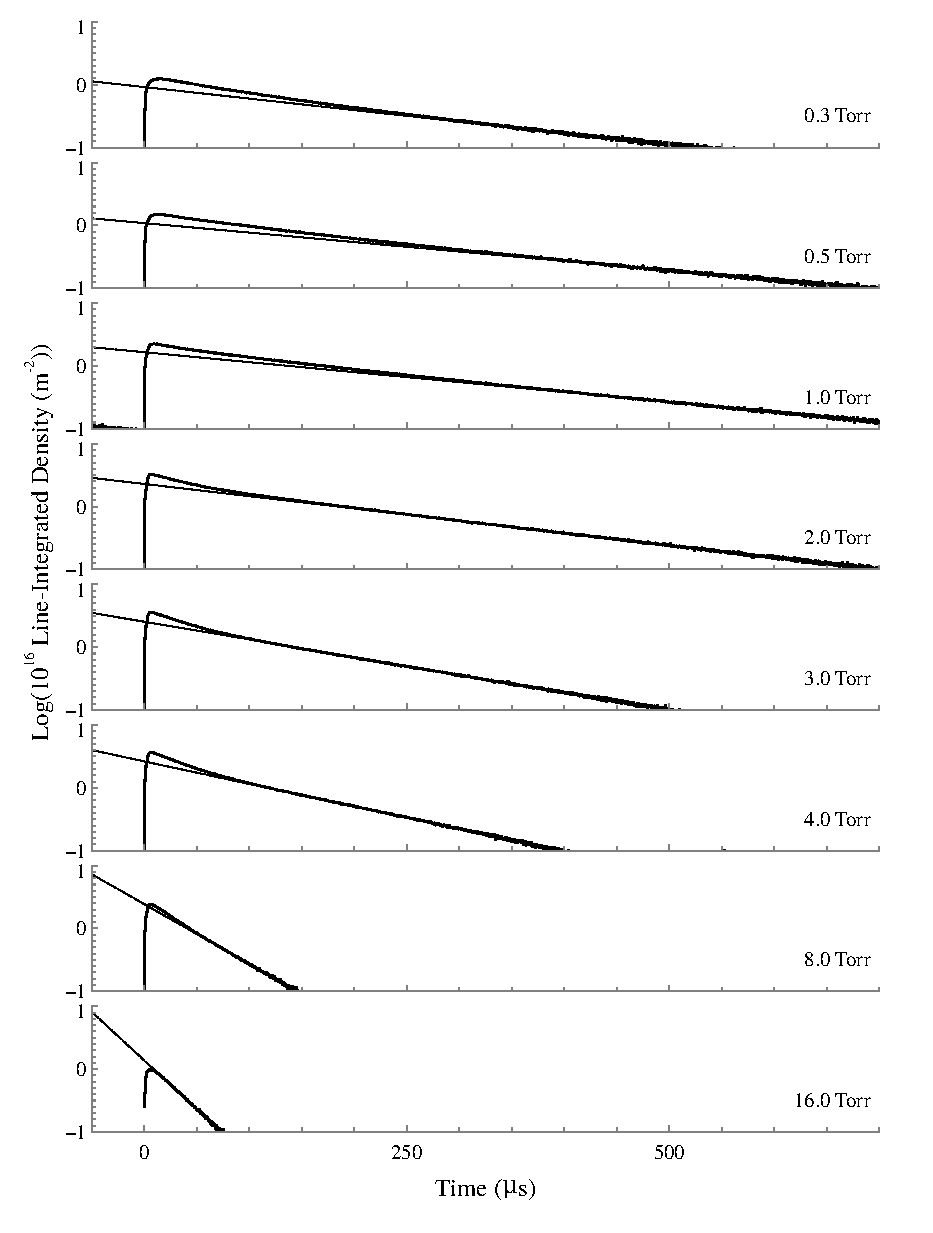
\includegraphics{./chapters/metastables/figures/long.eps}
  \caption{Measurements of the long-duration metastable density trends.
  Exponential fits are indicated by the dotted lines.}
  \label{fig:long}
\end{figure}
show the evolution of the metastables over time for each operating condition.


The long term metastable trends were measured for each pressure at the midstream
location


\subsection{Radial Density Maps}



With the exception of the data from the downstream location at low pressures,
these results are among the first direct measurements of \acs{rpnd} properties
on timescales relevant to its formation. The final temporal resolution was
determined by the photodiode, with a rise time of approximately 5 ns. 

  
  \chapter{Modeling}\label{chp:modeling}
    The measurements of the metastable dynamics may be used to better understand the
development of the \acs{rpnd} by the use of a plasma model. Working from the
metastable densities, it may be possible to predict electron characteristics,
such as temperature, density, as well as the densities of other excited states.
The ideal model would solve the Boltzmann equation (equation~\ref{eq:boltzmann})
for each species, over the entire geometry, in all dimensions, for as long as
was required to reach equilibrium.

Unfortunately, these requirements are somewhat problematic. Scale lengths of 10
$\mu$m are required in order to resolve the sheath effects, resulting in
approximately $2\times10%{13}$ spatial cells. Conservatively, the time steps
would be about 1 ns in length. At a minimum, the system required about five
minutes to reach equilibrium, thus necessitating $3\times10^{11}$ solution
steps. The largest velocity can be estimated as an electron accelerated across
the full applied potential (6.6 keV), and the lowest velocity would be room
temperature (0.04 eV). This produces a velocity discretization of about
$6\times10^7$ cells. Thus the size of the parameter space in question is about
$3.6\times10^{32}$. Given that the fastest computer in the world operates at 39
petaflops, a calculation of this magnitude would take around 0.3 billion years.
Of course, this is for only a single particle species, the total number in the
system is runs in the dozens (not including the impurities).

\section{Model Development}

It should be apparent that the Boltzmann equation must be simplified in order to
model the system in a reasonable amount of time. As discussed in
chapter~\ref{chp:theory}, the most common approach to this is the use of moments
of the Boltzmann equation which drastically simplifies the velocity terms.
Frequently, the moments of the Boltzmann equation are used to develop various
fluid approximations for plasmas \cite{Chen1984} (e.g.\ the two fluid equations,
the magnetohydrodynamic equations, etc.). This approach has been tremendously
successful in the description of everything from plasma display panels
\cite{Rauf1999b} to interstellar plasmas \cite{Linde1998}.

There are some limitation to the capabilities of these fluid descriptions. For
one, they require some assumption on the form of the \acs{eedf}. Often, the
distribution is assumed to be a Maxwell-Boltzmann or Druyvesteyn, depending on
the plasma conditions. In others, an approximate solution of the Boltzmann
equation may be used to tabulate rate coefficients as a function of the mean
energy \cite{Hagelaar2005}. In addition to this issue of the \acs{eedf}, fluid
models in large or complex geometries can still be quite computationally
expensive. This can limit the number of species and reactions which can be
addressed \cite{Lieberman2005}.

In order to obtain an estimate of the detailed dynamics which occur as the
\acs{rpnd} develops, it is necessary to consider additional simplifications of
the Boltzmann equation. One such possibility is the use of a global model where
the spatial dependence of the plasma parameters is assumed. This allows global
model simulations to ignore the geometry of the system and focus on the particle
interactions for long periods of time with reasonable computational
requirements.



The metastable measurements from the previous chapter showed little axial
variation for the majority of the operating conditions. Radial variations in the
emission intensity and excited state density have been observed
\cite{Vasilyak1994, Weatherford}, however the mechanism for this is poorly
understood.



\section{Distribution Effects}

\section{Pulse Shape Changes}

\section{Plasma Parameters}

\section{Summary}



  \chapter{Population Kinetics}\label{chp:emissions}

  \chapter{Conclusions}\label{chp:conclusions}

  \appendix
    \chapter{Millimeter-Wave Interferometry}\label{chp:mmw}
      \begin{equation}
  e = mc^2
\end{equation}

    \chapter{Rotational Spectroscopy}\label{chp:oes}
      Previous studies have found that ionization waves can induce fast gas heating in
molecular gas systems \cite{Popov2011}. Up to 40\% of the input energy can be
converted into translational energy through dissociation of oxygen and quenching
or electronically excited nitrogen states. In combustion applications, this gas
heating can play an important role in the combustion chemistry, flame holding,
and ignition delay. Likewise, gas heating can impact material processing and
ionization efficiency in other \acs{rpnd} applications. As such, it is important
to develop reliable temperature diagnostics for \acs{rpnd}s in molecular gases.

As early as 2001, researchers have proposed the use of a novel, hybrid engine
design for use in supersonic and hypersonic flight \cite{Macheret2001}. Like an
earlier program which advertised the use of a magnetohydrodynamic (\acs{mhd})
accelerator for controlling the gas inlet of a scramjet \cite{Gurijanov1996}.
Essentially, a hypersonic flow would be ionized by some external source, and
used as the working fluid in a downstream \acs{mhd} generator. The electrical
power produced by this system could be used for onboard electronics and
subsequent acceleration stages. The slowed flow could then be used with a
traditional turbojet engine.

One of the primary difficulties in the development of this \acs{mhd} energy
bypass engine was the efficient ionization of the inlet flow. Originally,
Macheret suggested the use of electron beams, carefully tuned to coincide with
the peak in the ionization cross section. However, the use of electron beams in
the ionization of high pressure gases is accompanied by a large number of
technical issues, similar to those some excimer lasers. Therefore, in 2006,
Nishihara et al.\ proposed the use of an \acs{rpnd} to produce an ``electron
beam'' in situ \cite{Nishihara2006}.



\section{Experiment}


\section{Theory}



Researchers at have proposed the use of a novel hybrid engine for supersonic and
hypersonic flight \cite{}.

The measurement of rotational spectra has been used several


  \bibliographystyle{unsrt}
  \bibliography{./Thesis}

\end{document}
